% created on 28/07/2020
% @author : ebazan
%\part{Image Contours}\label{part:image_contours}
%
%\section*{Introduction}
%We remember that the thesis's general objective is to propose vision-based algorithms for UAVs' navigation aid. Drone navigation is a complex task, so we propose decomposing the problem into concrete and straightforward tasks.  We consider that scene understanding is an essential aspect in image analysis for the robot navigation problem. Then, the proposal is to build a framework that obtains perceptual information using low-level primitives and low-level features of the image. The idea is to attack the first stages of scene understanding and object recognition tasks: detecting and identifying objects.  
%
%In this chapter of the thesis, we focus on studying the the intensity information in an image and their properties. We review some concepts of human perception, such as Helmholtz's principle, and we interpret and apply them to the contours extracted from the intensity information.  More specifically, we use the non-accidentalness (\textit{a contrario} approach) of the image contours to avoid modeling the possible objects to detect. Instead, we detect objects as a deviation of the normality represented by a random configuration model. This approach is inspired by postulates of works from the beginning of the 20th century that we strive to formalize mathematically. We use this algorithm for the autonomous drone landing task. Therefore, the objects to be identified are a series of numbered landing targets specifically designed for this problem.
%
%The main contributions of this chapter are:
%
%\begin{enumerate}
%	\item Study and comparison of different classical approaches to image contours detection.
%	\item A new methodology for searching and interpreting perceptual information using the a contrario method and Gestalt theory.
%	\item A non-parametric framework for fully unsupervised landing target detection robust to the image degradations present in the autonomous landing task.
%	\item An algorithm coding information into landing targets.
%
%\end{enumerate}


%\chapter{Unsupervised Object Detection for UAV Autonomous Landing Task} \label{ch:landing_target_detection}
\chapter{Intensity Image Contours and Information's Perceptual Organization} \label{ch:landing_target_detection}
%Associated publications: \vspace{-2mm}
%
%\begin{itemize}
%	\item \citep{Bazan.Dokladal.ea:ACIVS:2018}. << Unsupervised Perception Model for UAVs Landing Target Detection and Recognition >>. In: \textit{International Conference on Advanced Concepts for Intelligent Vision Systems}. Springer, pp 233-244.
%	\item \citep{Bazan.Dokladal.ea:RFIAP:2018}. << Non supervised perceptual model for target recognition in UAVs >>. In: \textit{Reconnaissance des Formes, Image, Apprentissage et Perception RFIAP}, Marne la Vallée, France.
%\end{itemize}

\section*{Résumé}
\noindent Dans ce chapitre, nous abordons le problème de l'atterrissage autonome des drones, et plus précisément, la détection et la reconnaissance robustes d'une cible d'atterrissage unique dans un environnement extérieur. Le défi est de savoir comment gérer les images dans des conditions de lumière non contrôlées, impactées par des ombres, le changement d'échelle, la perspective, les vibrations, le bruit, le flou, entre autres. Nous introduisons un modèle robuste non supervisé qui nous permet de détecter et de reconnaître une cible de manière perceptuelle, en utilisant les principes de Gestalt de non-accidentalité et de regroupement. Notre modèle extrait les contours d'une cible d'atterrissage sous la forme de valeurs aberrantes à l'aide du détecteur d'anomalies RX et du calcul de la proximité et d'une mesure de similarité. Enfin, nous montrons le code Hamming de correction d'erreur pour générer des cibles d'atterrissage numérotées et réduire les erreurs de reconnaissance.

\section*{Abstract}
\noindent In this chapter, we tackle the problem of UAV's autonomous landing, and more precisely, the robust detection and recognition of a unique landing target in an outdoor environment. The challenge is how to deal with images under non-controlled light conditions impacted by shadows, change of scale, perspective, vibrations, noise, blur, among others. We introduce a robust unsupervised model that allows us to detect and recognize a target in a perceptual-inspired manner, using the Gestalt principles of non-accidentalness and grouping. Our model extracts the landing target contours as outliers using the RX anomaly detector and computing proximity and a similarity measure. Finally, we show the error correction Hamming code to generate numbered landing targets and reduce the recognition errors.


\section{Introduction}\label{sec:introduction_ch1}
We remember that the thesis's general objective is to propose vision-based algorithms for UAVs' navigation aid. Drone navigation is a complex task, so we propose decomposing the problem into concrete and straightforward tasks.  We consider that scene understanding is an essential aspect in image analysis for the robot navigation problem. Then, the proposal is to build a framework that obtains perceptual information using low-level primitives and low-level features of the image. The idea is to attack the first stages of scene understanding and object recognition tasks: detecting and identifying objects.  

In this chapter of the thesis, we focus on studying the the intensity information in an image and their properties. We review some concepts of human perception, such as Helmholtz's principle, and we interpret and apply them to the contours extracted from the intensity information.  More specifically, we use the non-accidentalness (\textit{a contrario} approach) of the image contours to avoid modeling the possible objects to detect. Instead, we detect objects as a deviation of the normality represented by a random configuration model. This approach is inspired by postulates of works from the beginning of the 20th century that we strive to formalize mathematically. We use this algorithm for the autonomous drone landing task. Therefore, the objects to be identified are a series of numbered landing targets specifically designed for this problem.

The main contributions of this chapter are:

\begin{enumerate}
	\item Study and comparison of different classical approaches to image contours detection.
	\item A new methodology for searching and interpreting perceptual information using the a contrario method and Gestalt theory.
	\item A non-parametric framework for fully unsupervised landing target detection robust to the image degradations present in the autonomous landing task.
	\item An algorithm coding information into landing targets.

\end{enumerate}

\subsection{Landing Target Detection Problems and State-of-the-Art}
Nowadays, the target detection for UAVs' autonomous landing is a recurring subject in the industrial sector. This task is crucial so that applications such as air parcel delivery can be developed. Some strategies to address this problem are creating landing stations; infrastructures that could harbor extra elements, such as GPS, infrared markers, or telecommunication sensors, which serve to locate and differentiate the landing zone from other areas. This option may be feasible for small-scale applications; however, in applications that require multiple landing points, this becomes impractical.

Instead, we propose a monocular vision-based system for the detection and identification of custom landing targets. For this, we imagine the situation when a drone is ready to land as follows: first, the drone reaches a certain horizontal/vertical distance from a possible landing target, then it activates the visual system and analyzes the scene where there may be a target; if the drone recognizes a pattern as a landing target and the ID is correct, the drone lands. The figure \ref{fig:visionbased_landing_problem_sketch} represents the actions that a drone must perform to land at the correct point. The use of vision systems for target detection provides advantages such as the independence of special onboard sensors, such as IR cameras to detect infrared markers and the continuous operation in areas with low or no GPS coverage.

\begin{figure}[!ht]
    \centering
    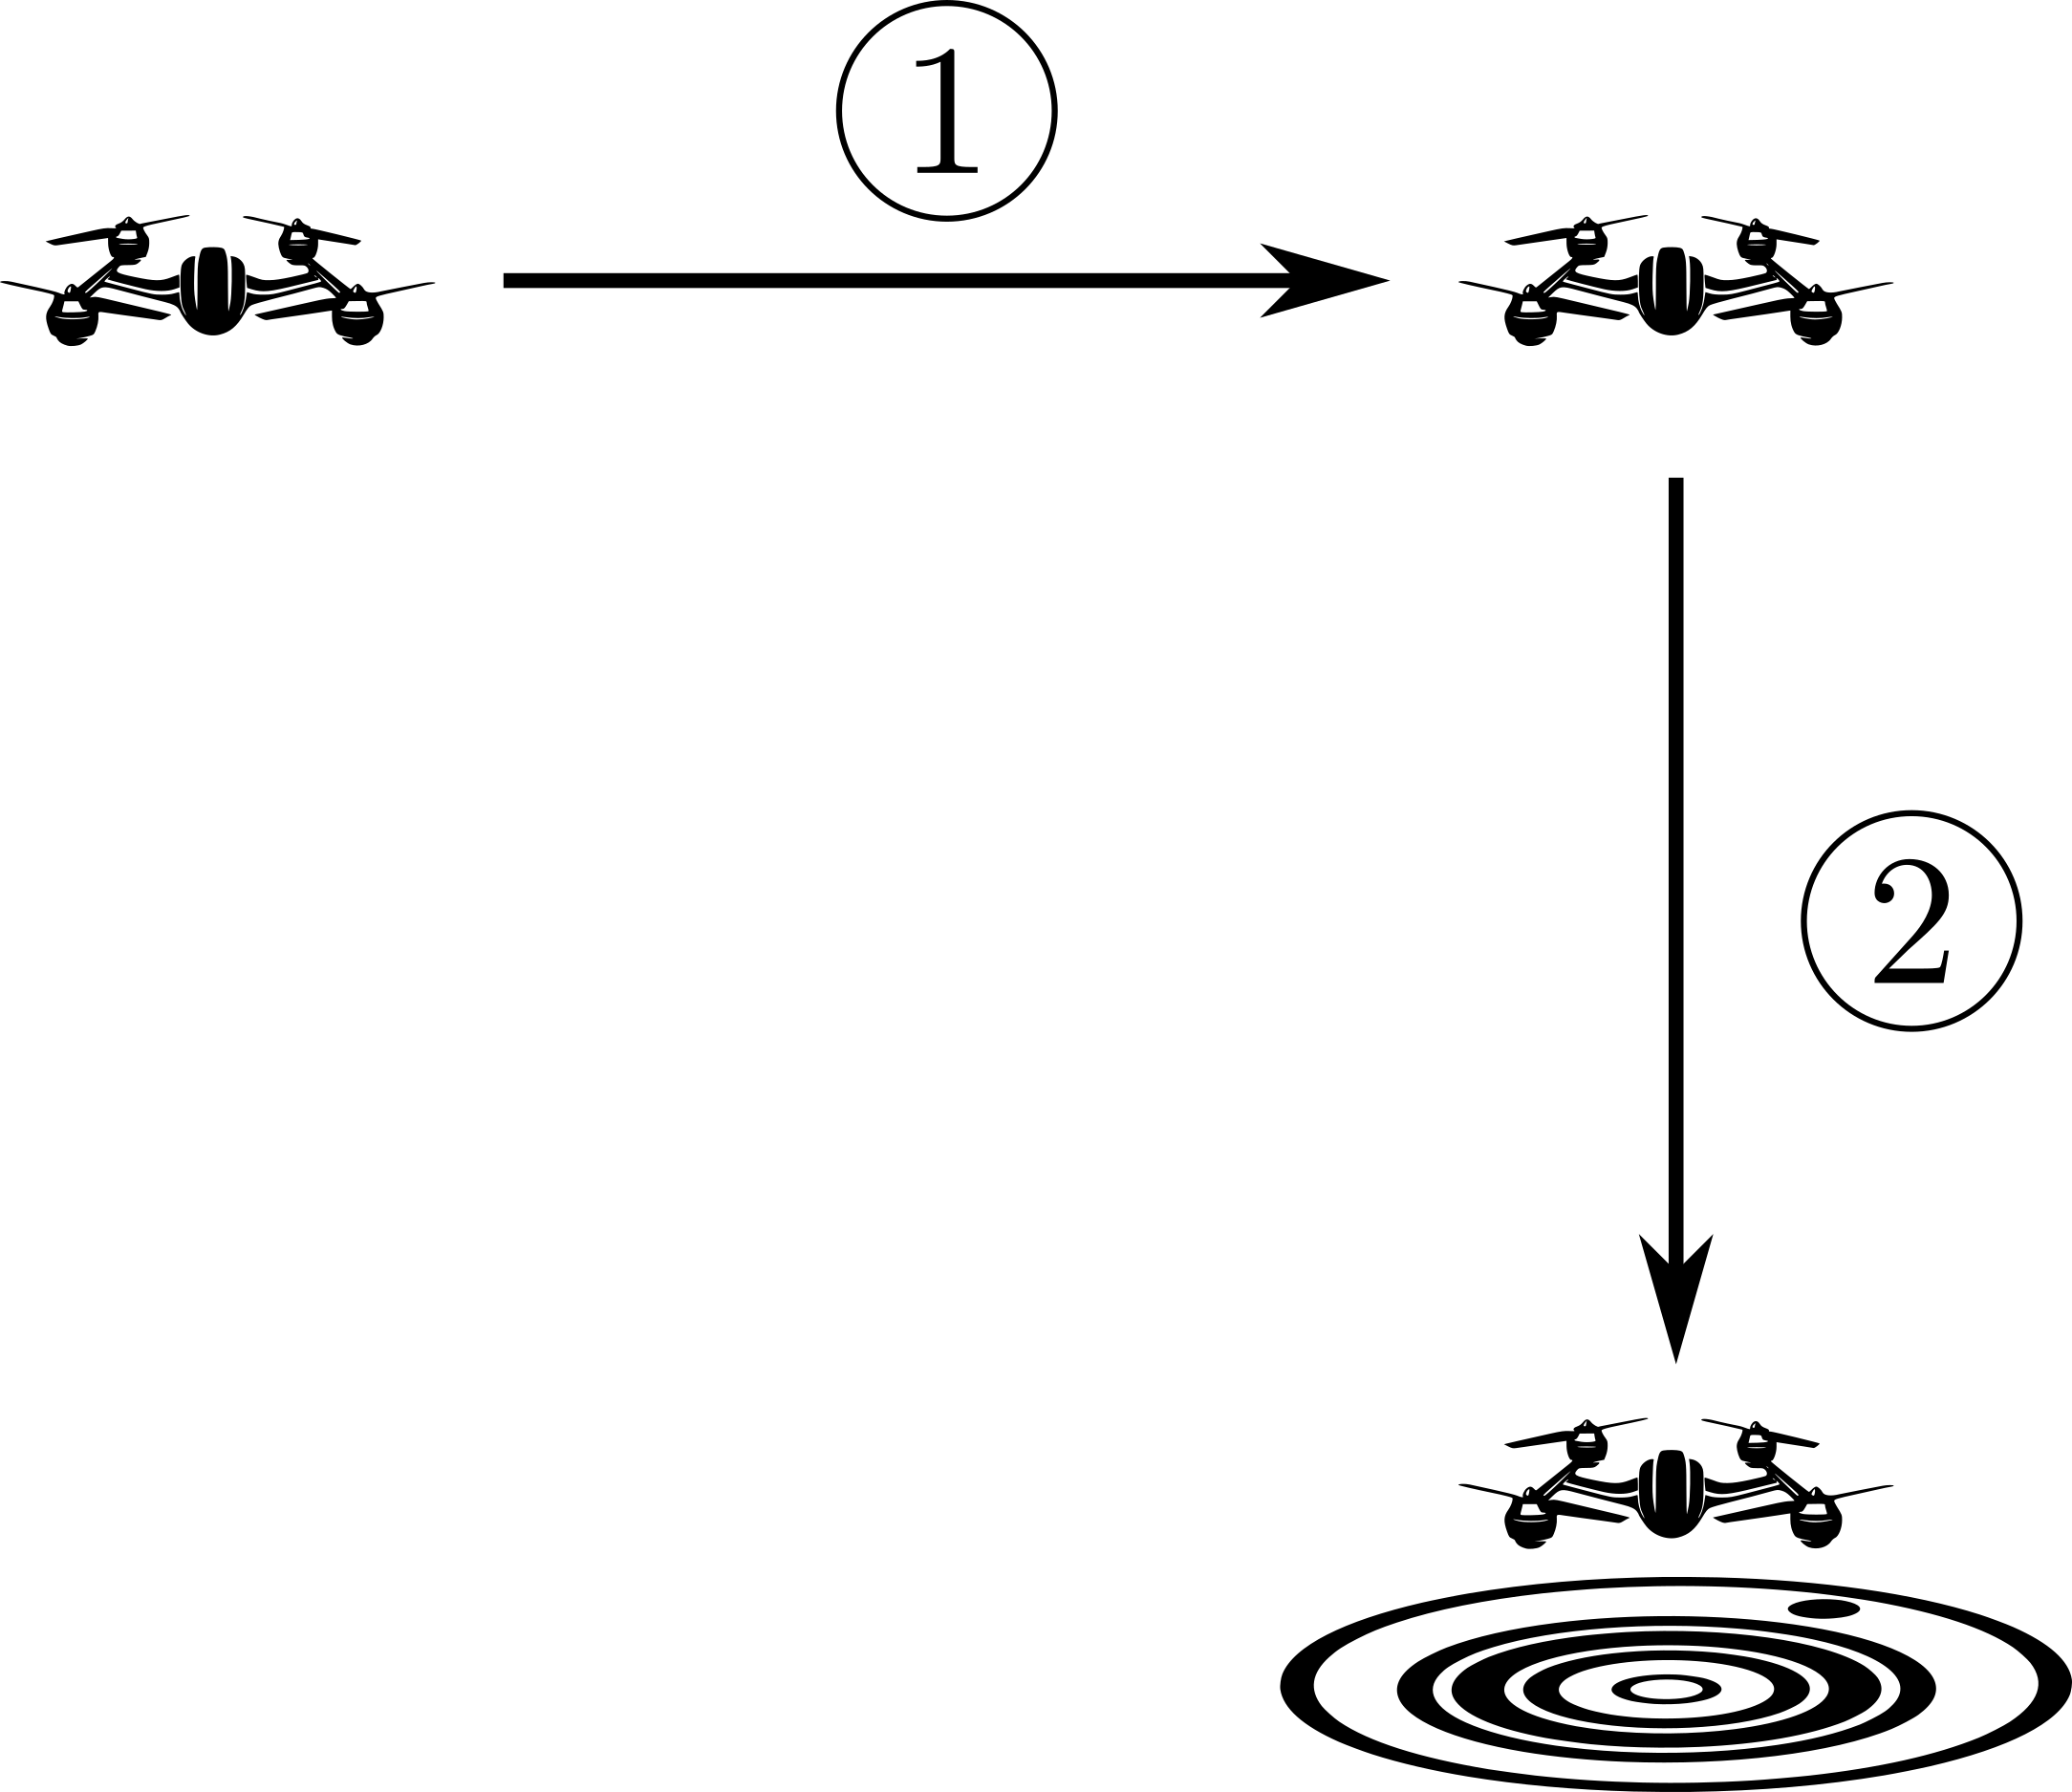
\includegraphics[width=0.5\textwidth]{problem_statement}        
    \caption{Graphic representation of the two stages involved in vision-based autonomous landing: 1. Approach to the landing zone; 2. Detection and recognition of the landing target.}\label{fig:visionbased_landing_problem_sketch}
\end{figure}

Notwithstanding, using visual systems in outdoor environments presents challenges as many uncontrolled variables affect and impair the object detection task. The main problems to face in the aerial landing target detection task are the non-controlled light changes that generate shadowing, reflectance, and saturation on the surfaces; the perspective and distance of the camera that deforms the objects; the motion and vibrations that blur the images and; the noise generated by a low-quality sensor.

The landing target detection can be viewed as an image segmentation problem, where there is a wide range of developed methods. The variational framework \citep{Mumford.Shah:CPAM:1989}, offers an optimal general method for image segmentation; however, its mathematical complexity and the endless selection of fidelity and regularization parameters make its use complex. Also, the number of iterations needed to find the optimal solution makes it impossible to have real-time results. Conversely, threshold-based methods have been used to detect landing targets \citep{Lacroix.Caballero:IROS:2006}, \citep{Lange.Sunderhauf.ea:SIMPAR:2008} for their ease of use. However, to achieve good detection, their use is limited to indoor spaces, where the light conditions are controlled \citep{Araar.Aouf.ea:IROS:2017}. 

Recently, convolutional neural networks (CNN) techniques offer the possibility of detecting an object from a large set of classes with a high-reliability \citep{Carrio.Sampedro.ea:JS:2017}. Nevertheless, we need to train CNN methods with a database containing the object classes in a wide range of situations, and, in case of changes in the object or the scene, the database must be rebuilt \citep{Yao.Yu.ea:CCC:2017}, \citep{Furukawa:TechRep:2018}. Besides, in some cases, the computation is carried out off-board the drone, which implies the need for network infrastructure and limitation of autonomy \citep{Lee.Wang.ea:IRC:2017}.

From a practical point of view, we can interpret landing targets as fiducial markers. However, fiducial markers are designed to serve as measurement or reference points into a scene. We can find in the literature different proposals for the automatic generation of fiducial markers and their respective detection algorithms \citep{Fiala:PAMI:2010}, \citep{Naimark.Foxlin:ISMAR:2002}. However, detection algorithms can fail for several reasons, such as poor lighting conditions, rapid camera movements, and occlusions. A common approach to improve the robustness of a marker detection system is the use of marker boards, i.e., a pattern composed of multiple markers \citep{Garrido-Jurado.Munoz-Salinas.ea:PR:2014}. 

We chose to design and detect our own landing targets using the image contours as input information and build a feature space. We then mathematically interpret the human perception concepts (Gestalt theory and Helmholtz principle) to find the landing targets as deviations of a random model.  With these elements, we detect the targets in an unsupervised way. We describe below such concepts and the different proven approaches to contour extraction and target identification.


\subsection{Conceptual Framework}
Humans can carry out the process of perception in a natural way \citep{Petitot:Neurogeometrie:2008}. We, as humans, identify meaningful features and exciting events in a scene (such as points, lines, edges, textures, colors, movement), and with the help of our memory and the learning capacity, we can recognize and classify objects. The identification of primitives is a consequence of their non-accidental apparition, i.e., they are not generated randomly \citep{Attneave:PR:1954}. This behavior is roughly the Helmholtz principle, which states that we do not perceive any structure in a uniform random image. However, whenever some deviation from randomness occurs, it is possible to find a structure. In other words, events that could not happen by chance are immediately perceived. This principle is represented in the figure \ref{fig:helmholtz_principle}.

\begin{figure}[!ht]
    \centering
    \begin{subfigure}[b]{0.25\textwidth}
        \includegraphics[width=\textwidth]{helmholtz_noise}
        \caption{}
        \label{fig:helmholtz_noise}
    \end{subfigure}
        ~ %add desired spacing between images, e. g. ~, \quad, \qquad, \hfill etc. 
      %(or a blank line to force the subfigure onto a new line)
    \begin{subfigure}[b]{0.25\textwidth}
        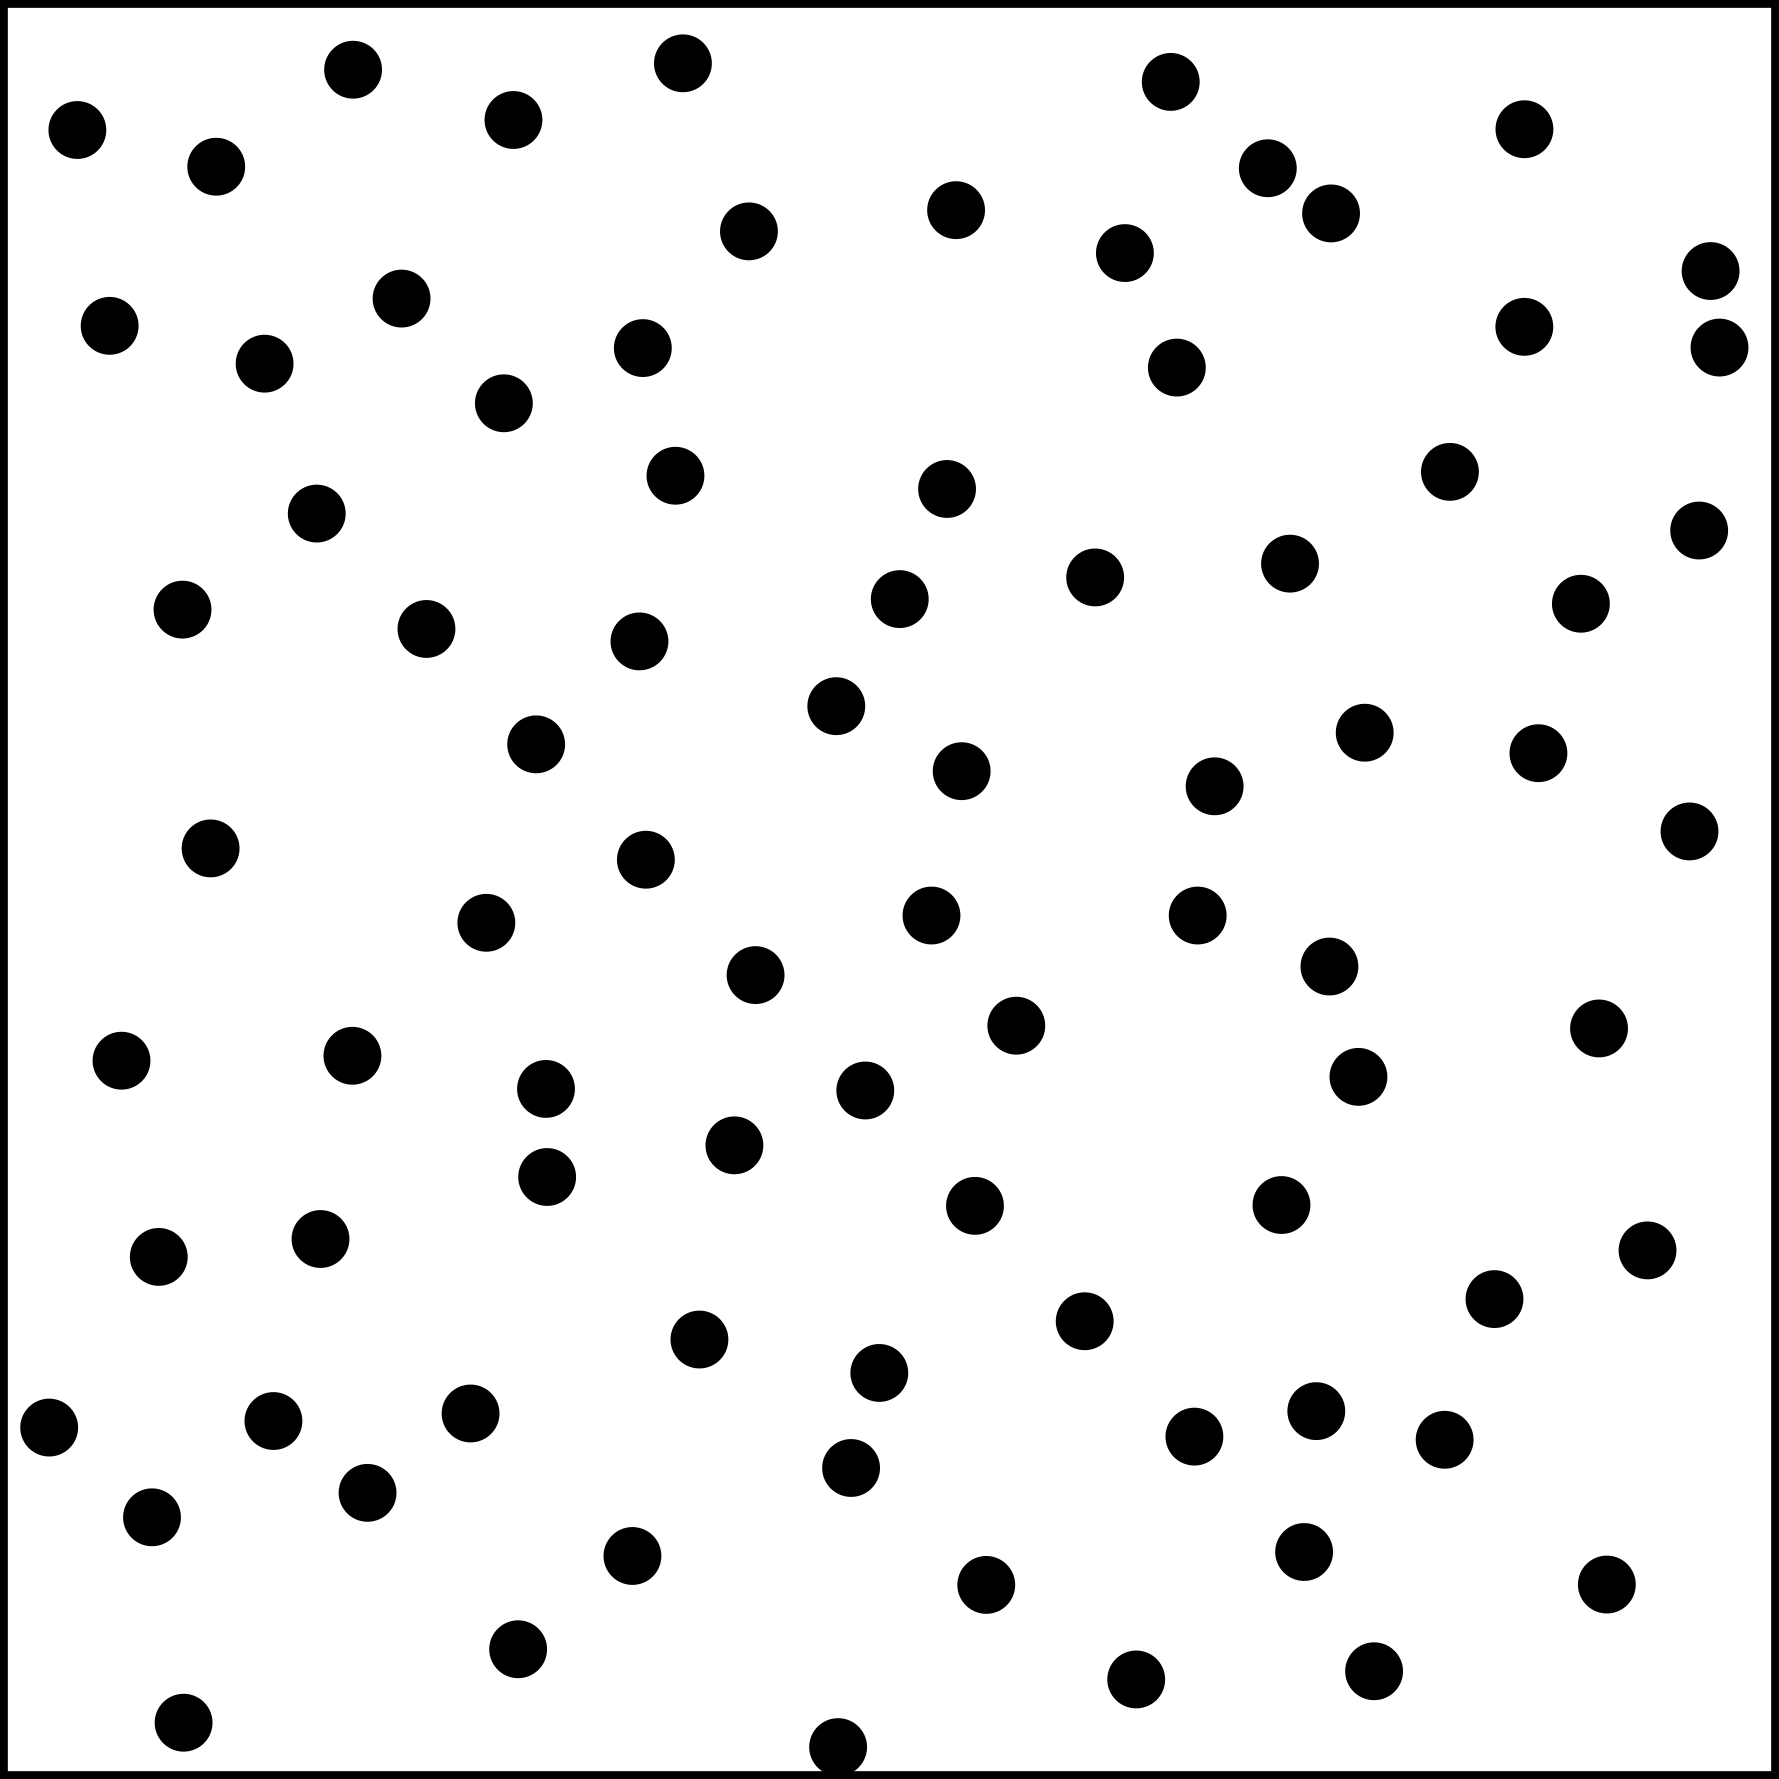
\includegraphics[width=\textwidth]{helmholtz_dots}
        \caption{}
        \label{fig:helmholtz_dots}
    \end{subfigure}
        ~ %add desired spacing between images, e. g. ~, \quad, \qquad, \hfill etc. 
      %(or a blank line to force the subfigure onto a new line)
    \begin{subfigure}[b]{0.25\textwidth}
        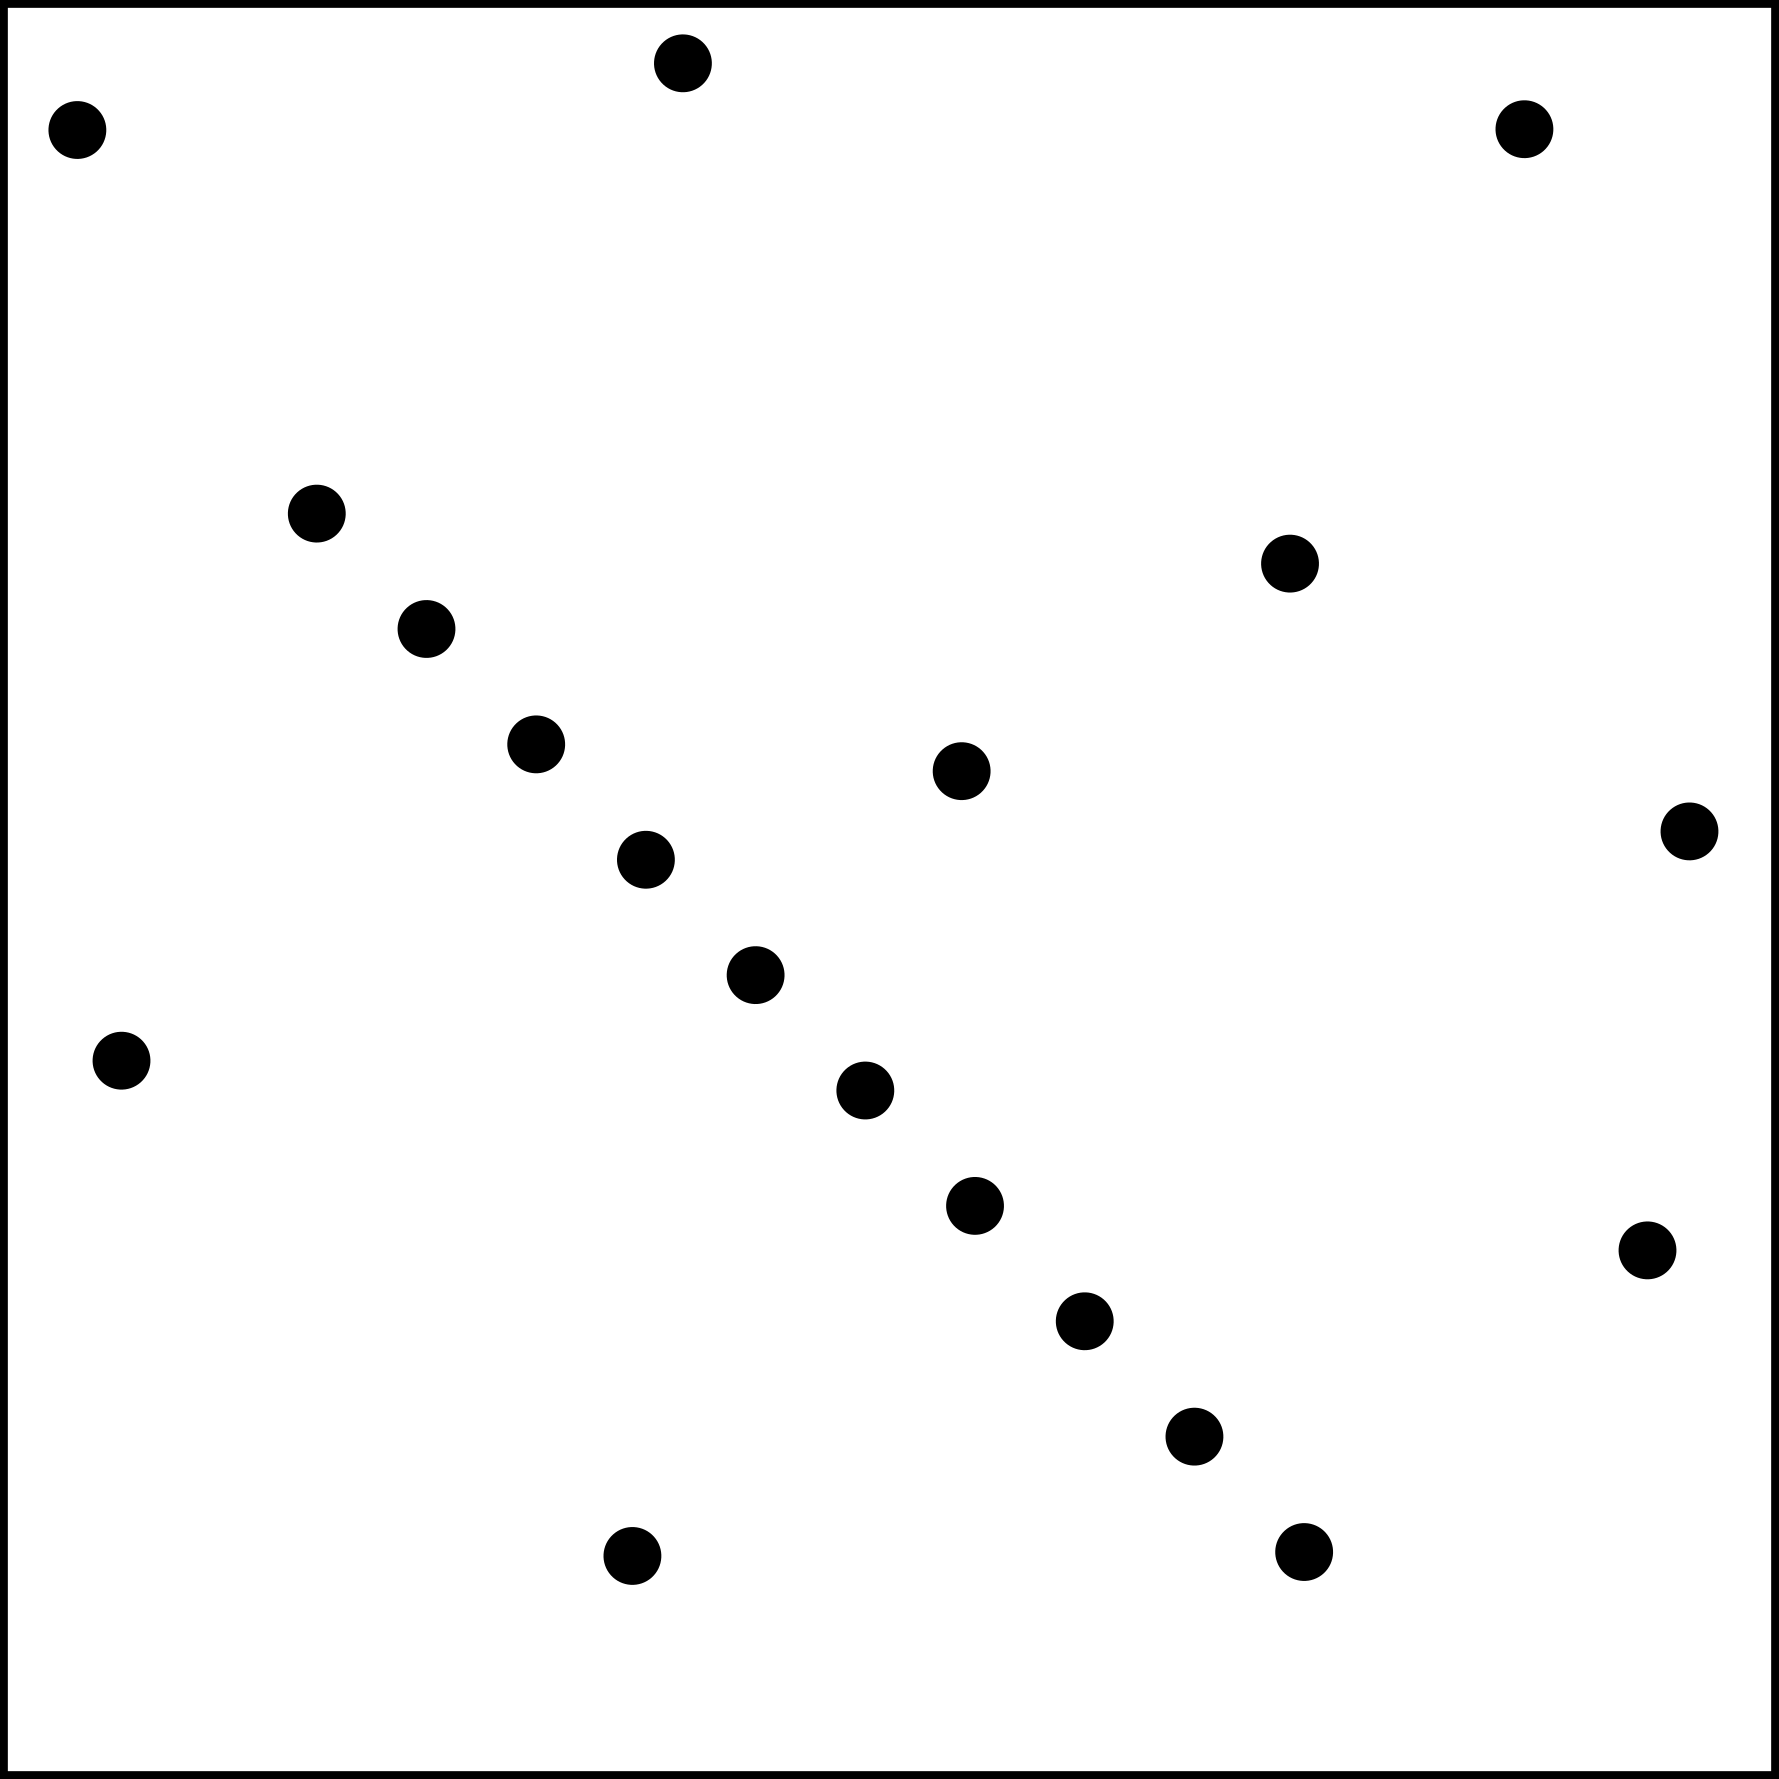
\includegraphics[width=\textwidth]{helmholtz_line}
        \caption{}
        \label{fig:helmholtz_line}
    \end{subfigure}
        
    \caption{Representation of Helmholtz's principle: \captext{(a)} Uniform random image where no structure can be found. A group of ten aligned dots exists in both images \captext{(b)}and \captext{(c)}, but this structure can hardly be seen in the central image. Otherwise, in the right-most image, the alignment stands out as a significant deviation from the randomness that cannot happen by chance and is therefore perceived.}\label{fig:helmholtz_principle}
\end{figure}

The Gestalt theory \citep{Wertheimer:Psycologische:1923} states that we can build a whole (a gestalt) through the grouping of non-accidental detected primitives. That means that the human mind recognizes objects as a whole before examining their individual parts, and the observer perceives the information that is not related in size, shape, or orientation as chaotic and disorganized. The grouping of individual elements in a whole follows a set of laws defined by the Gestalt theory; some of them are (see Fig. \ref{fig:gestalt_laws}):

\begin{itemize}
	\item Similarity law
	\item Proximity law
	\item Continuity law
	\item Closure law
	\item Connectedness law
	\item Figure-ground law	
\end{itemize}


\begin{figure}[!ht]
    \centering
    \begin{subfigure}[b]{0.25\textwidth}
        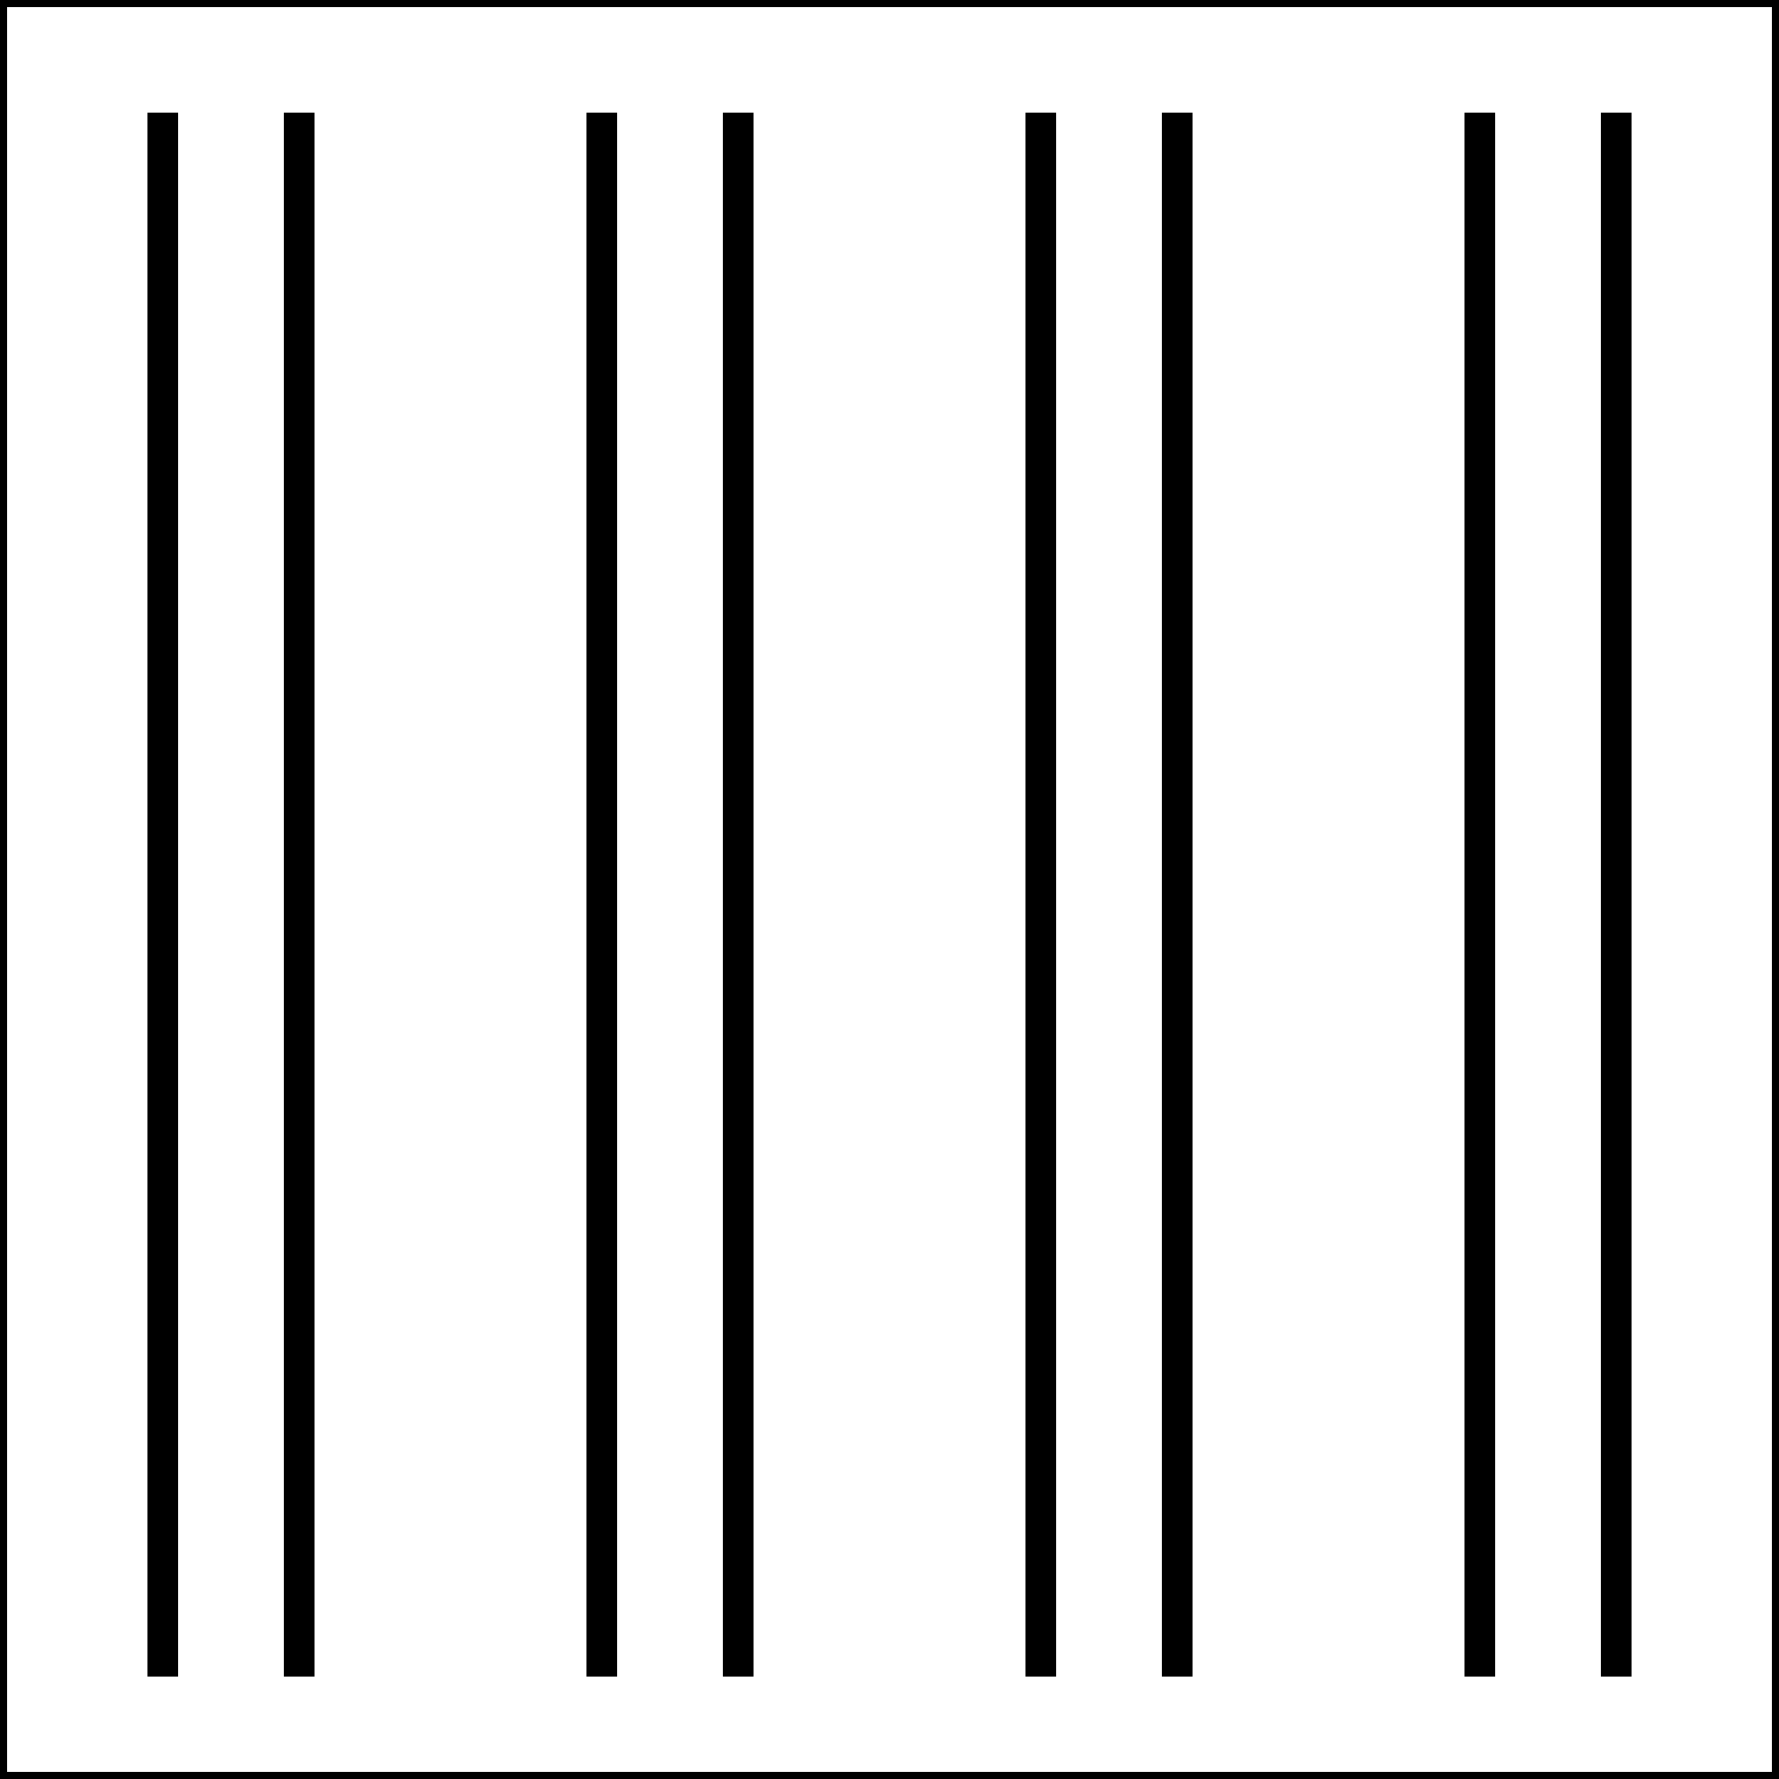
\includegraphics[width=\textwidth]{gestalt_proximity}
        \caption{Proximity}
        \label{fig:gestalt_proximity}
    \end{subfigure}
        ~ %add desired spacing between images, e. g. ~, \quad, \qquad, \hfill etc. 
      %(or a blank line to force the subfigure onto a new line)
    \begin{subfigure}[b]{0.25\textwidth}
        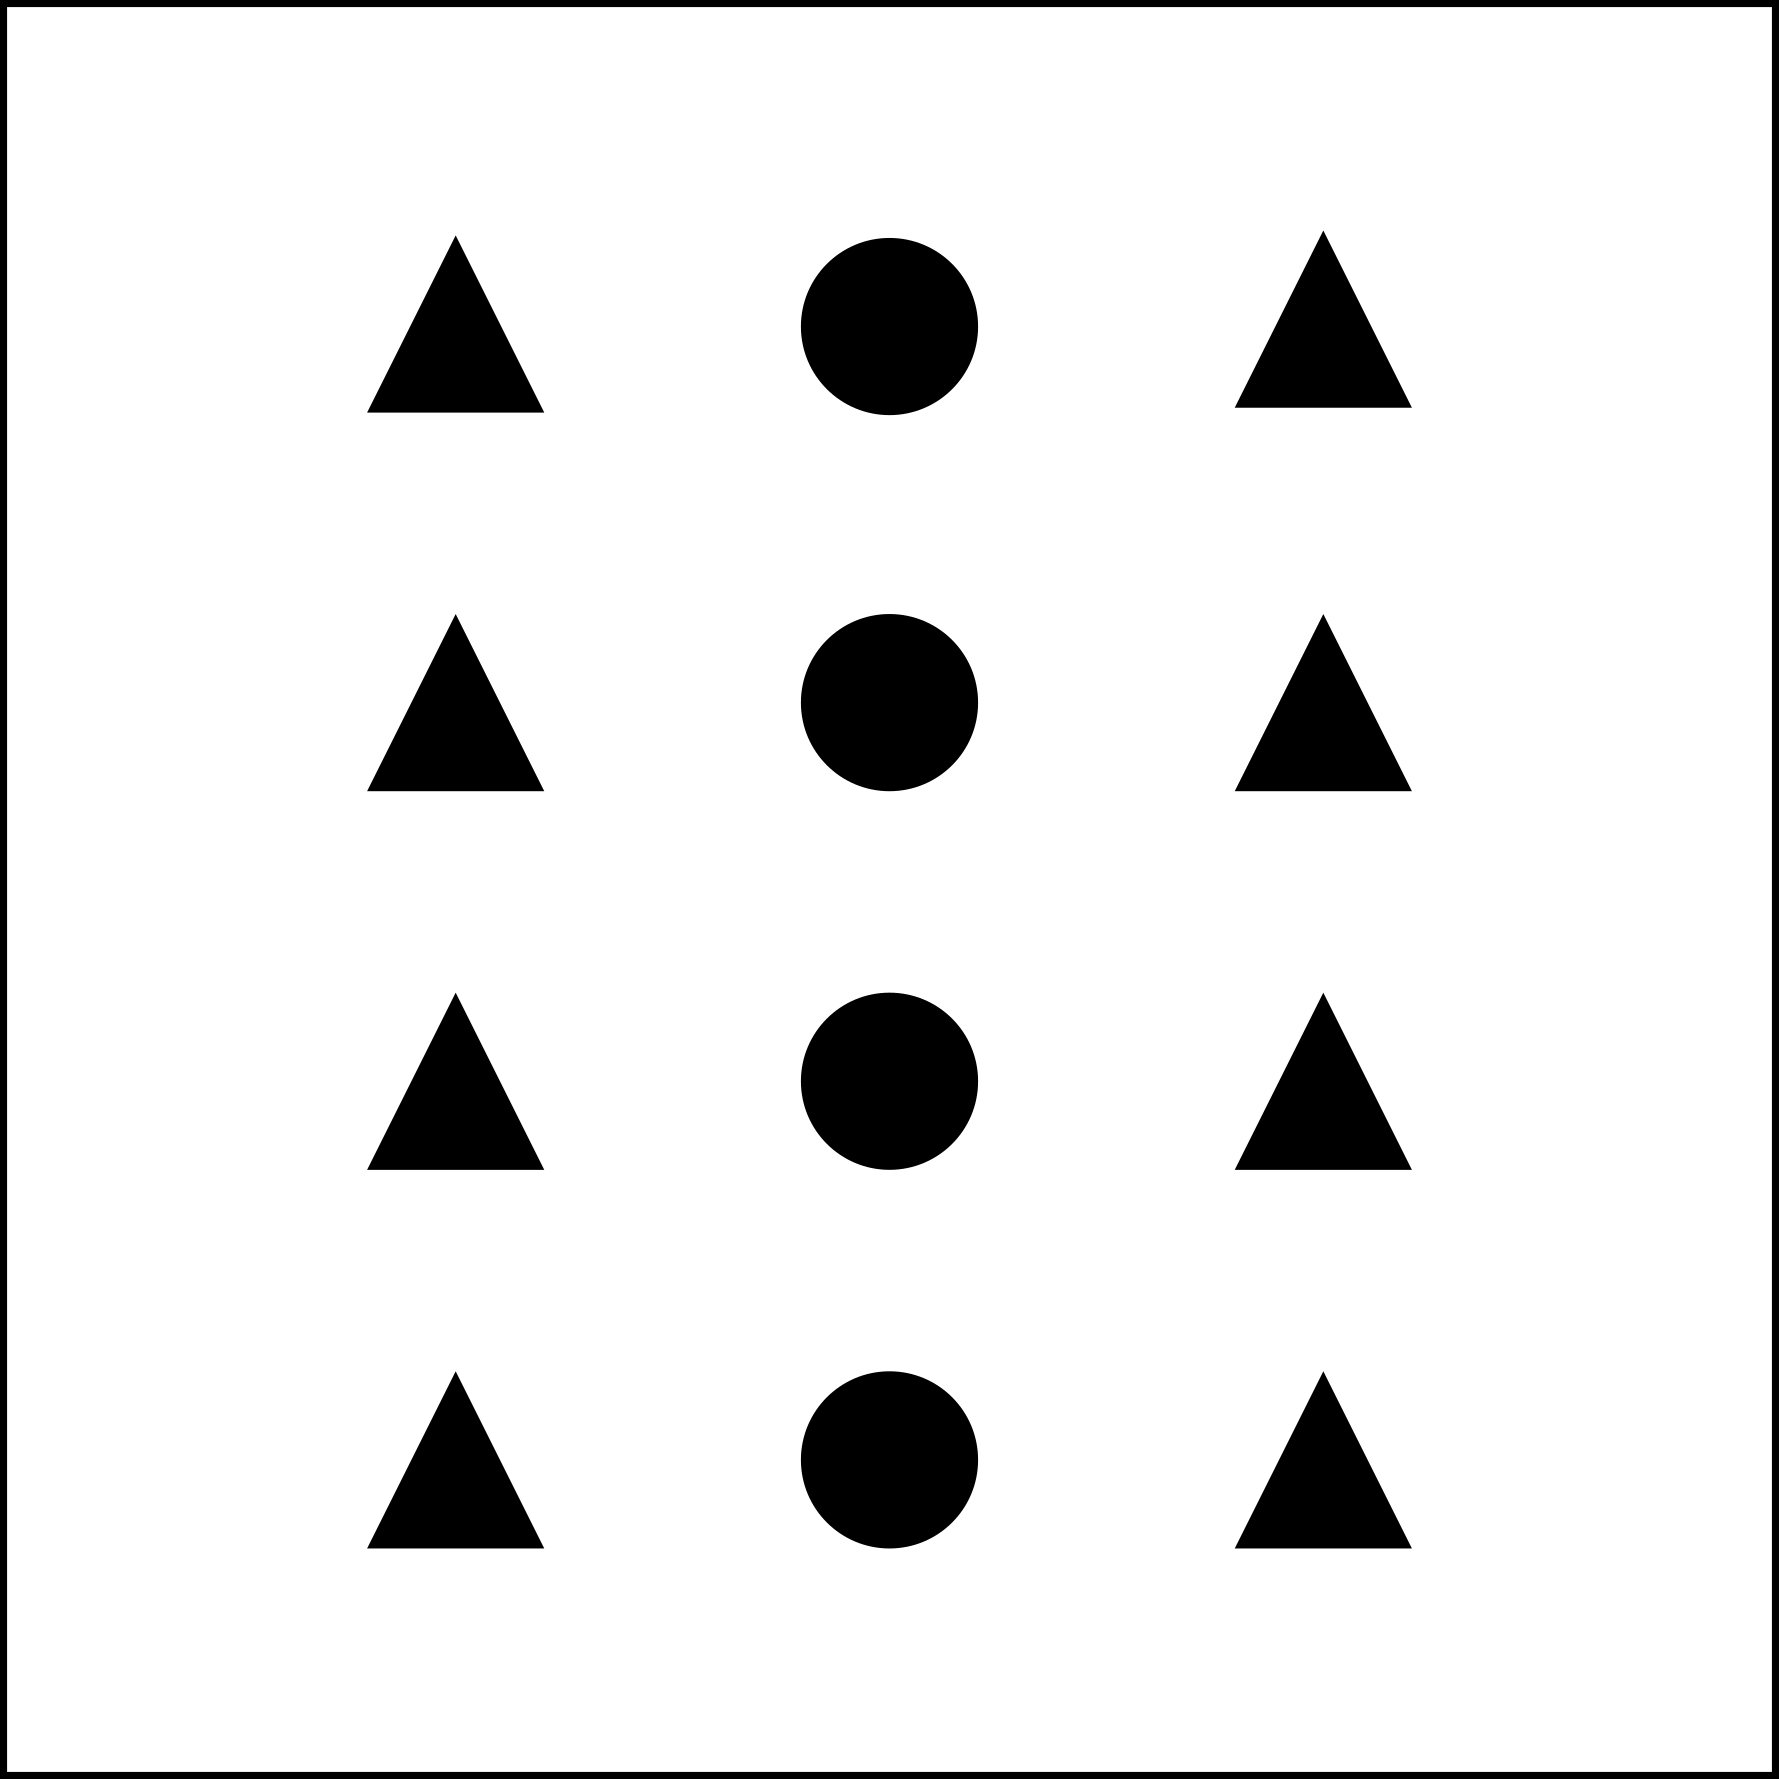
\includegraphics[width=\textwidth]{gestalt_similarity}
        \caption{Similarity}
        \label{fig:gestalt_similarity}
    \end{subfigure}
        ~ %add desired spacing between images, e. g. ~, \quad, \qquad, \hfill etc. 
      %(or a blank line to force the subfigure onto a new line)
    \begin{subfigure}[b]{0.25\textwidth}
        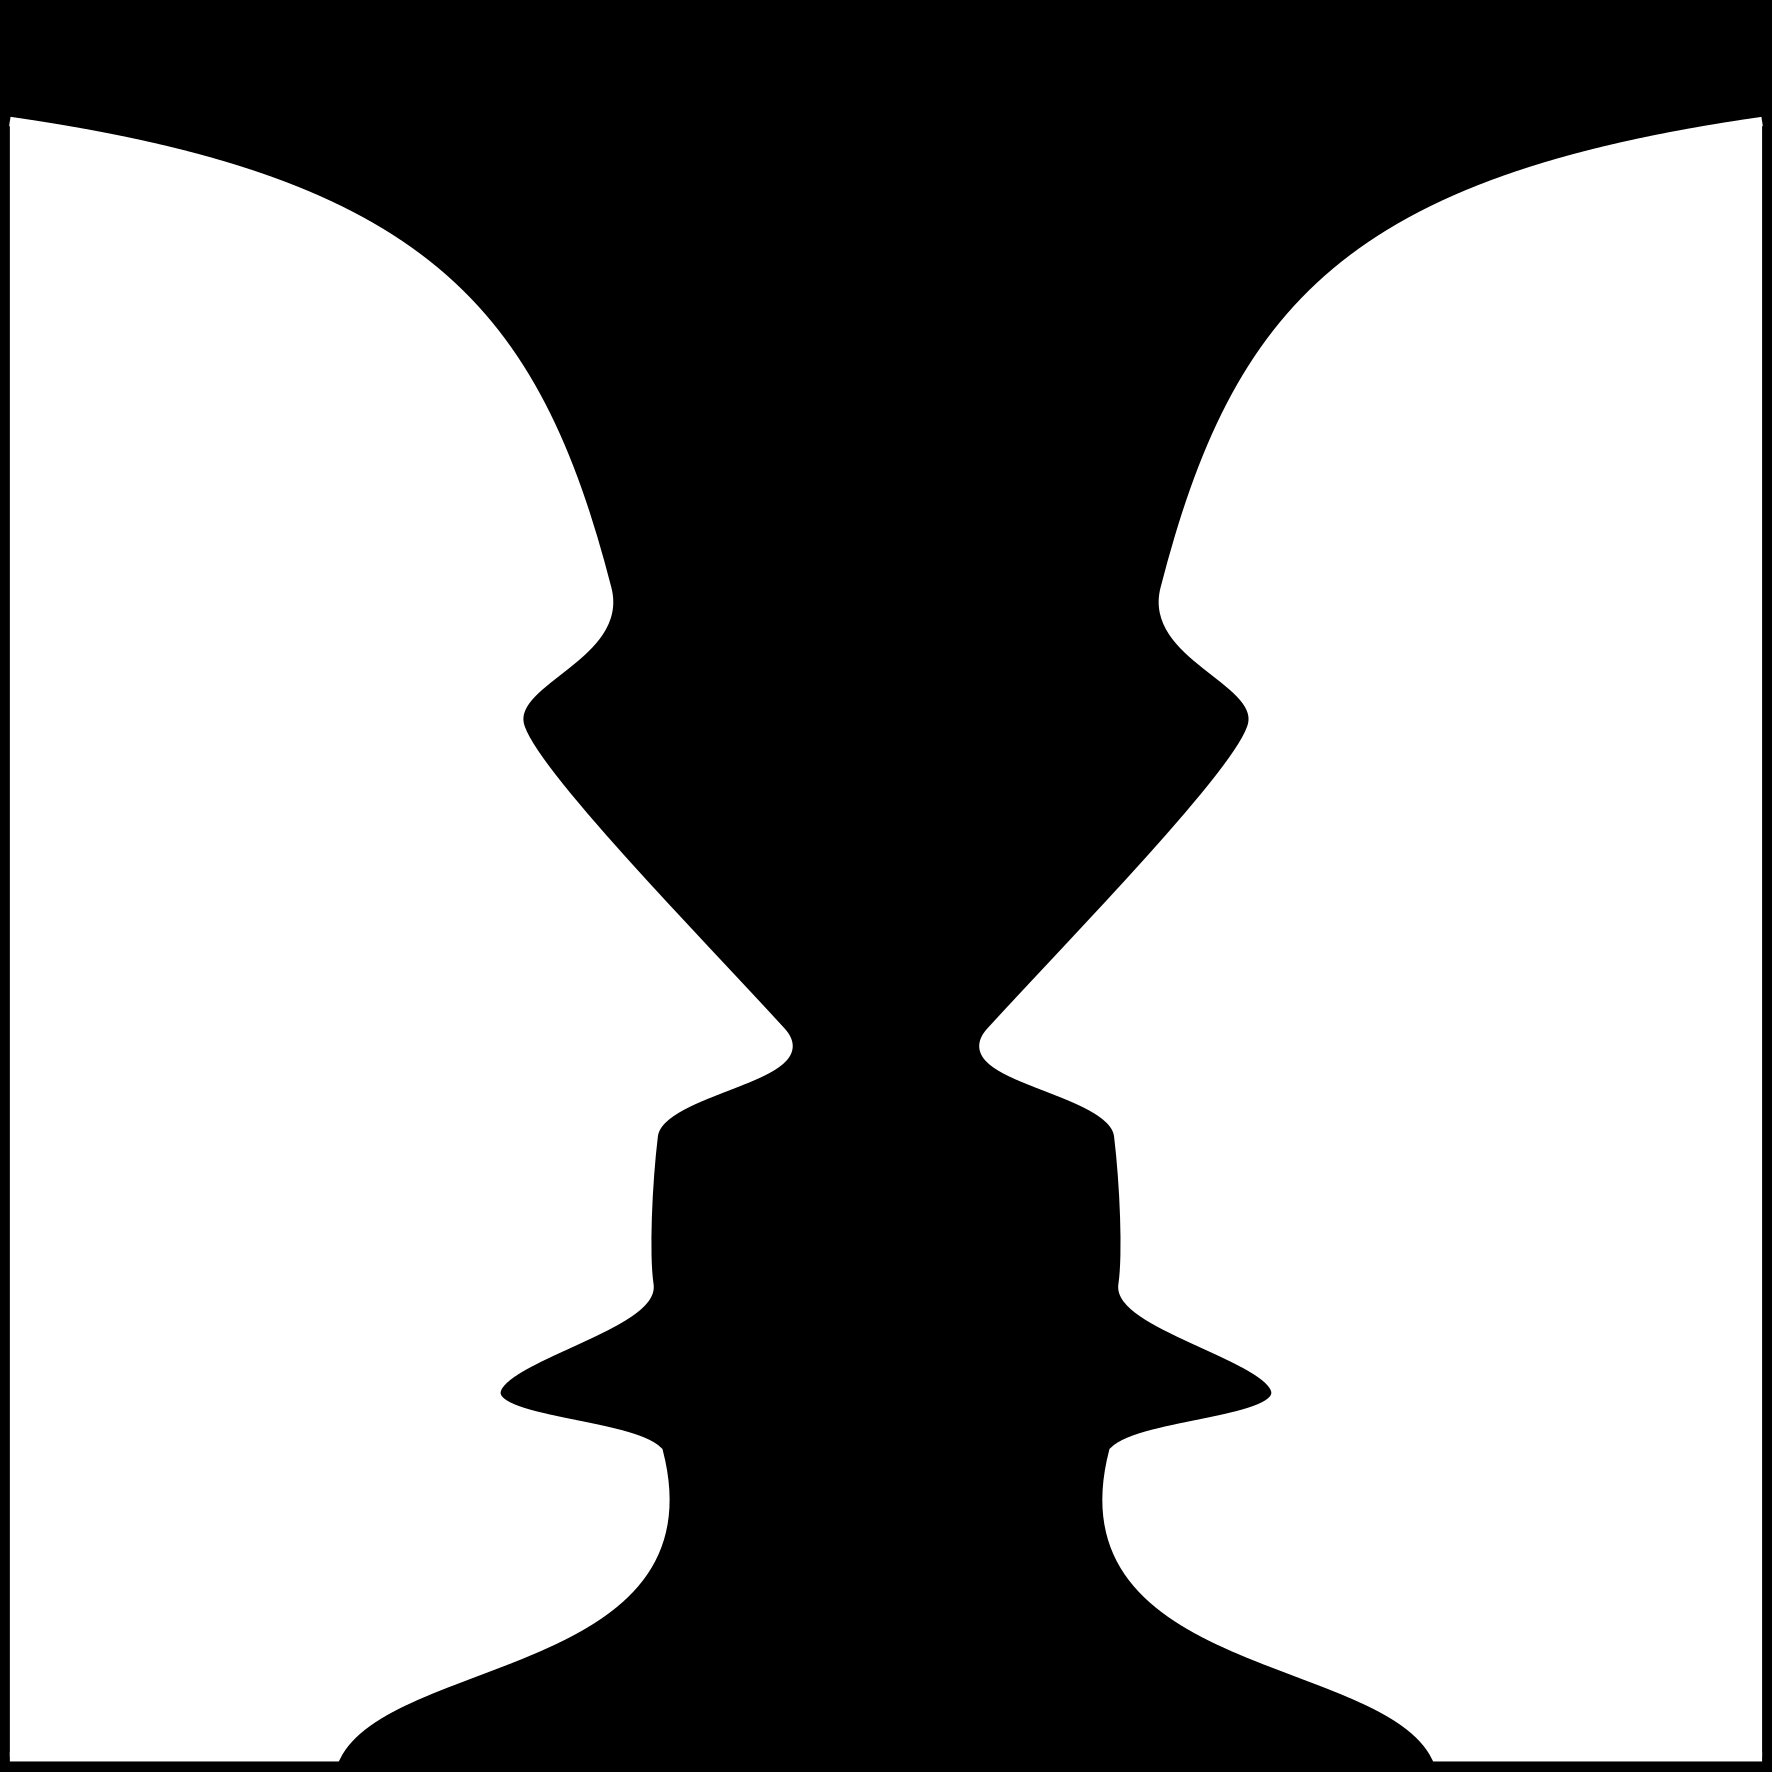
\includegraphics[width=\textwidth]{gestalt_figure_ground}
        \caption{Figure-ground}
        \label{fig:gestalt_figure_ground}
    \end{subfigure} \\
    \begin{subfigure}[b]{0.25\textwidth}
        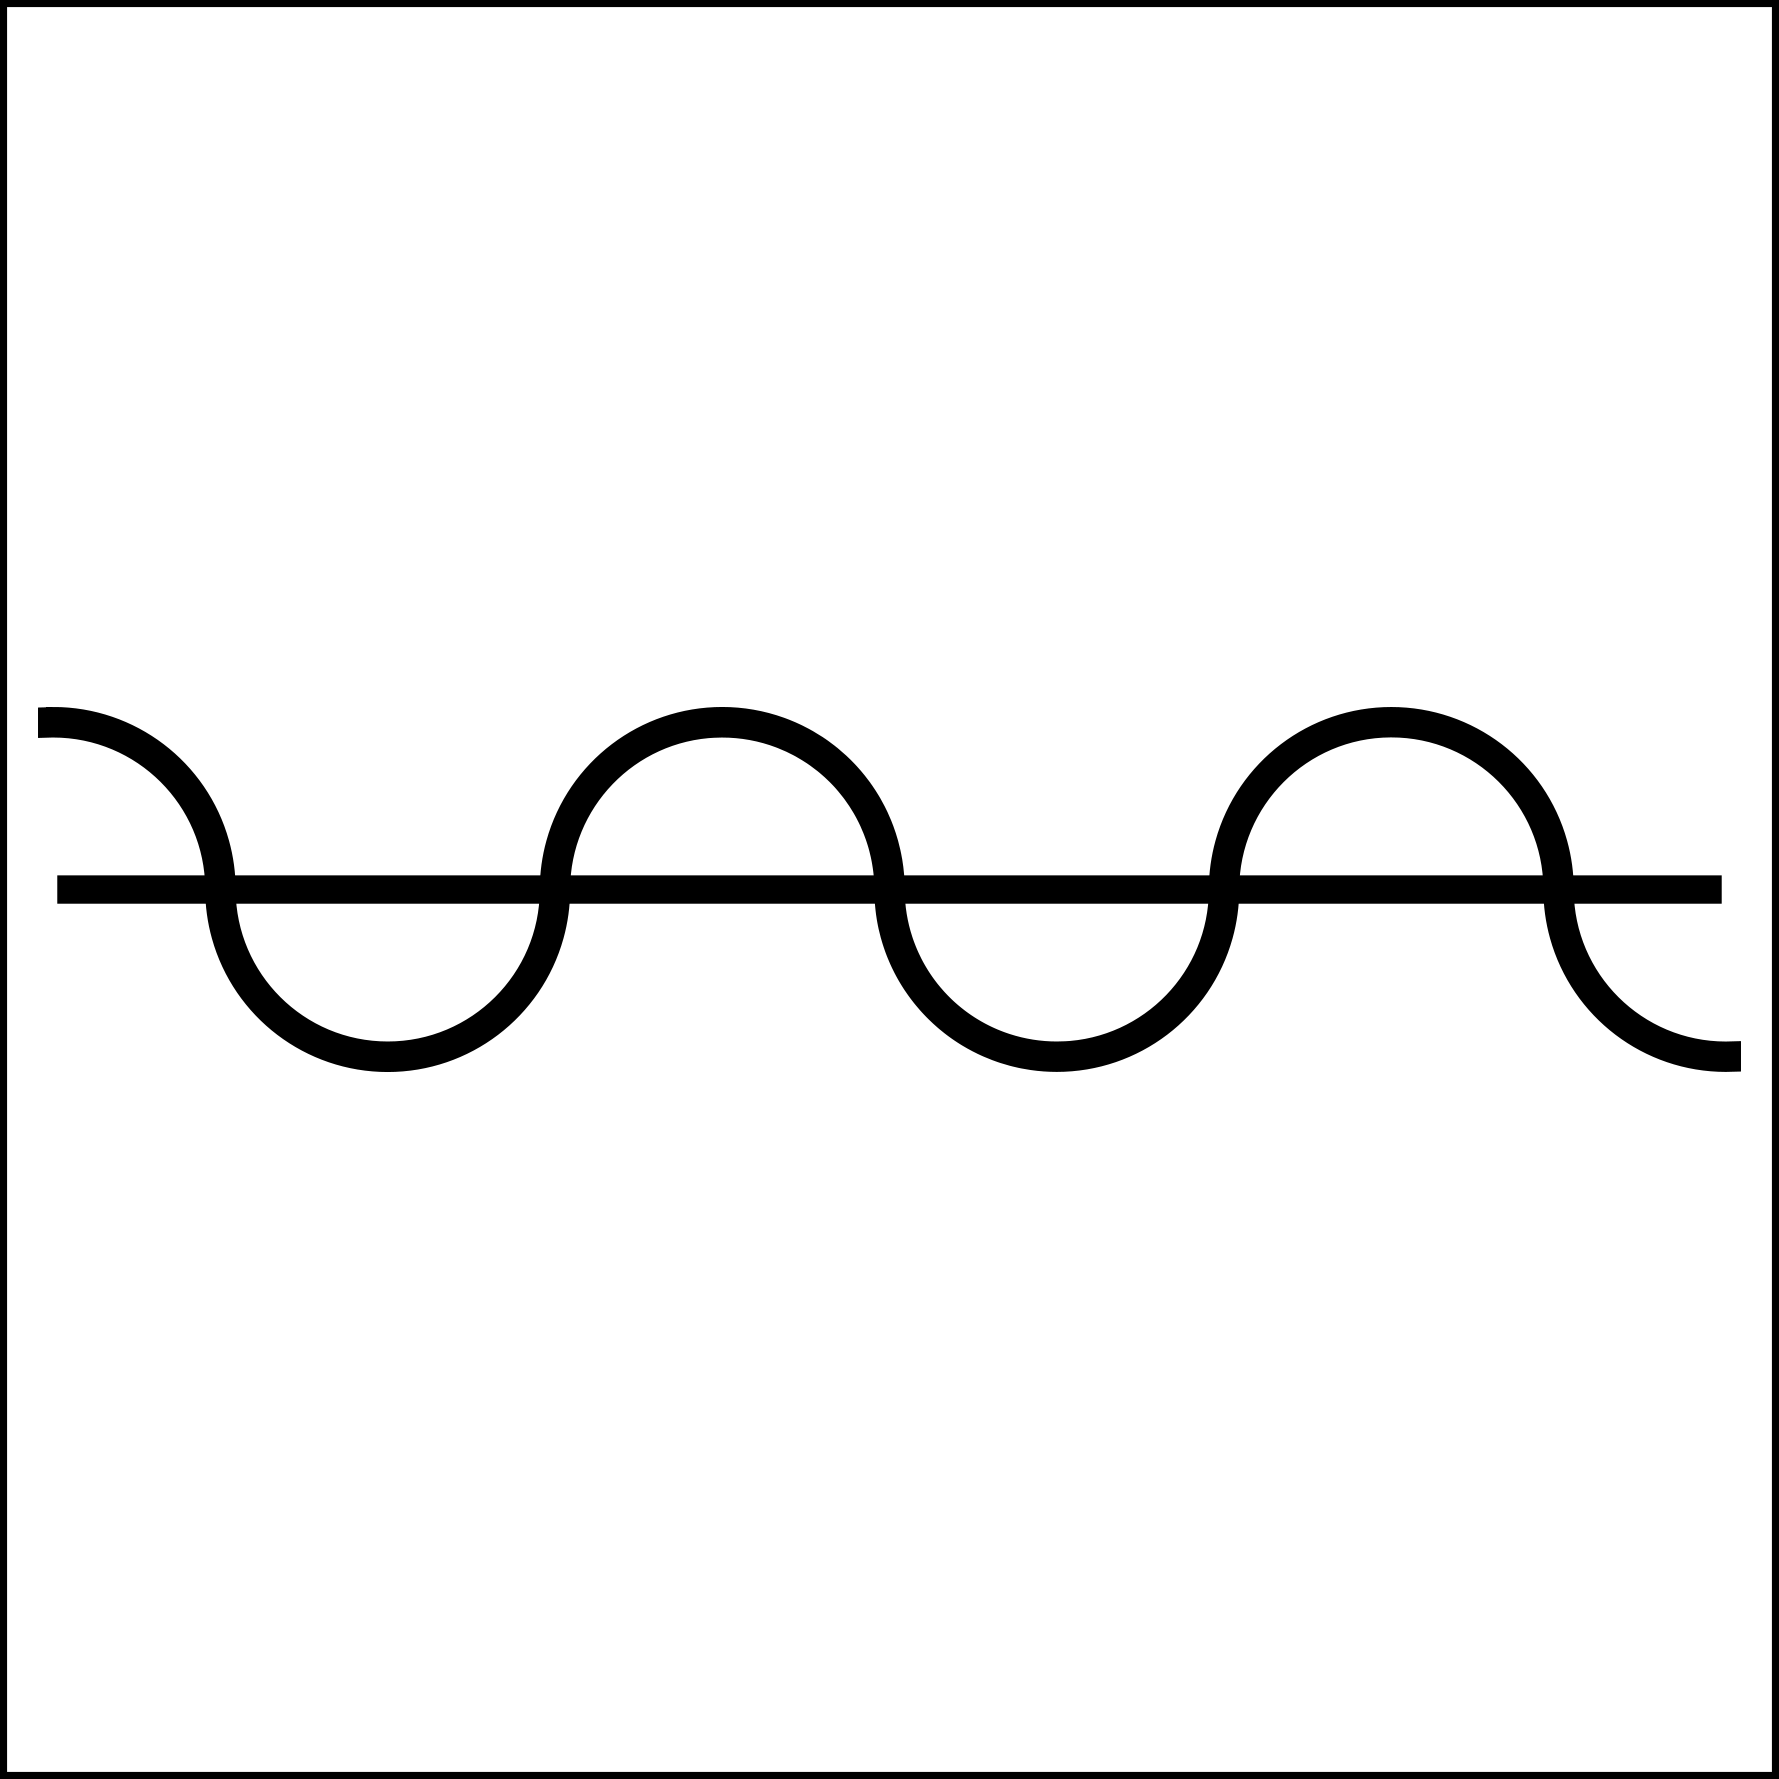
\includegraphics[width=\textwidth]{gestalt_continuity}
        \caption{Continuity}
        \label{fig:gestalt_continuity}
    \end{subfigure}
        ~ %add desired spacing between images, e. g. ~, \quad, \qquad, \hfill etc. 
      %(or a blank line to force the subfigure onto a new line)
    \begin{subfigure}[b]{0.25\textwidth}
        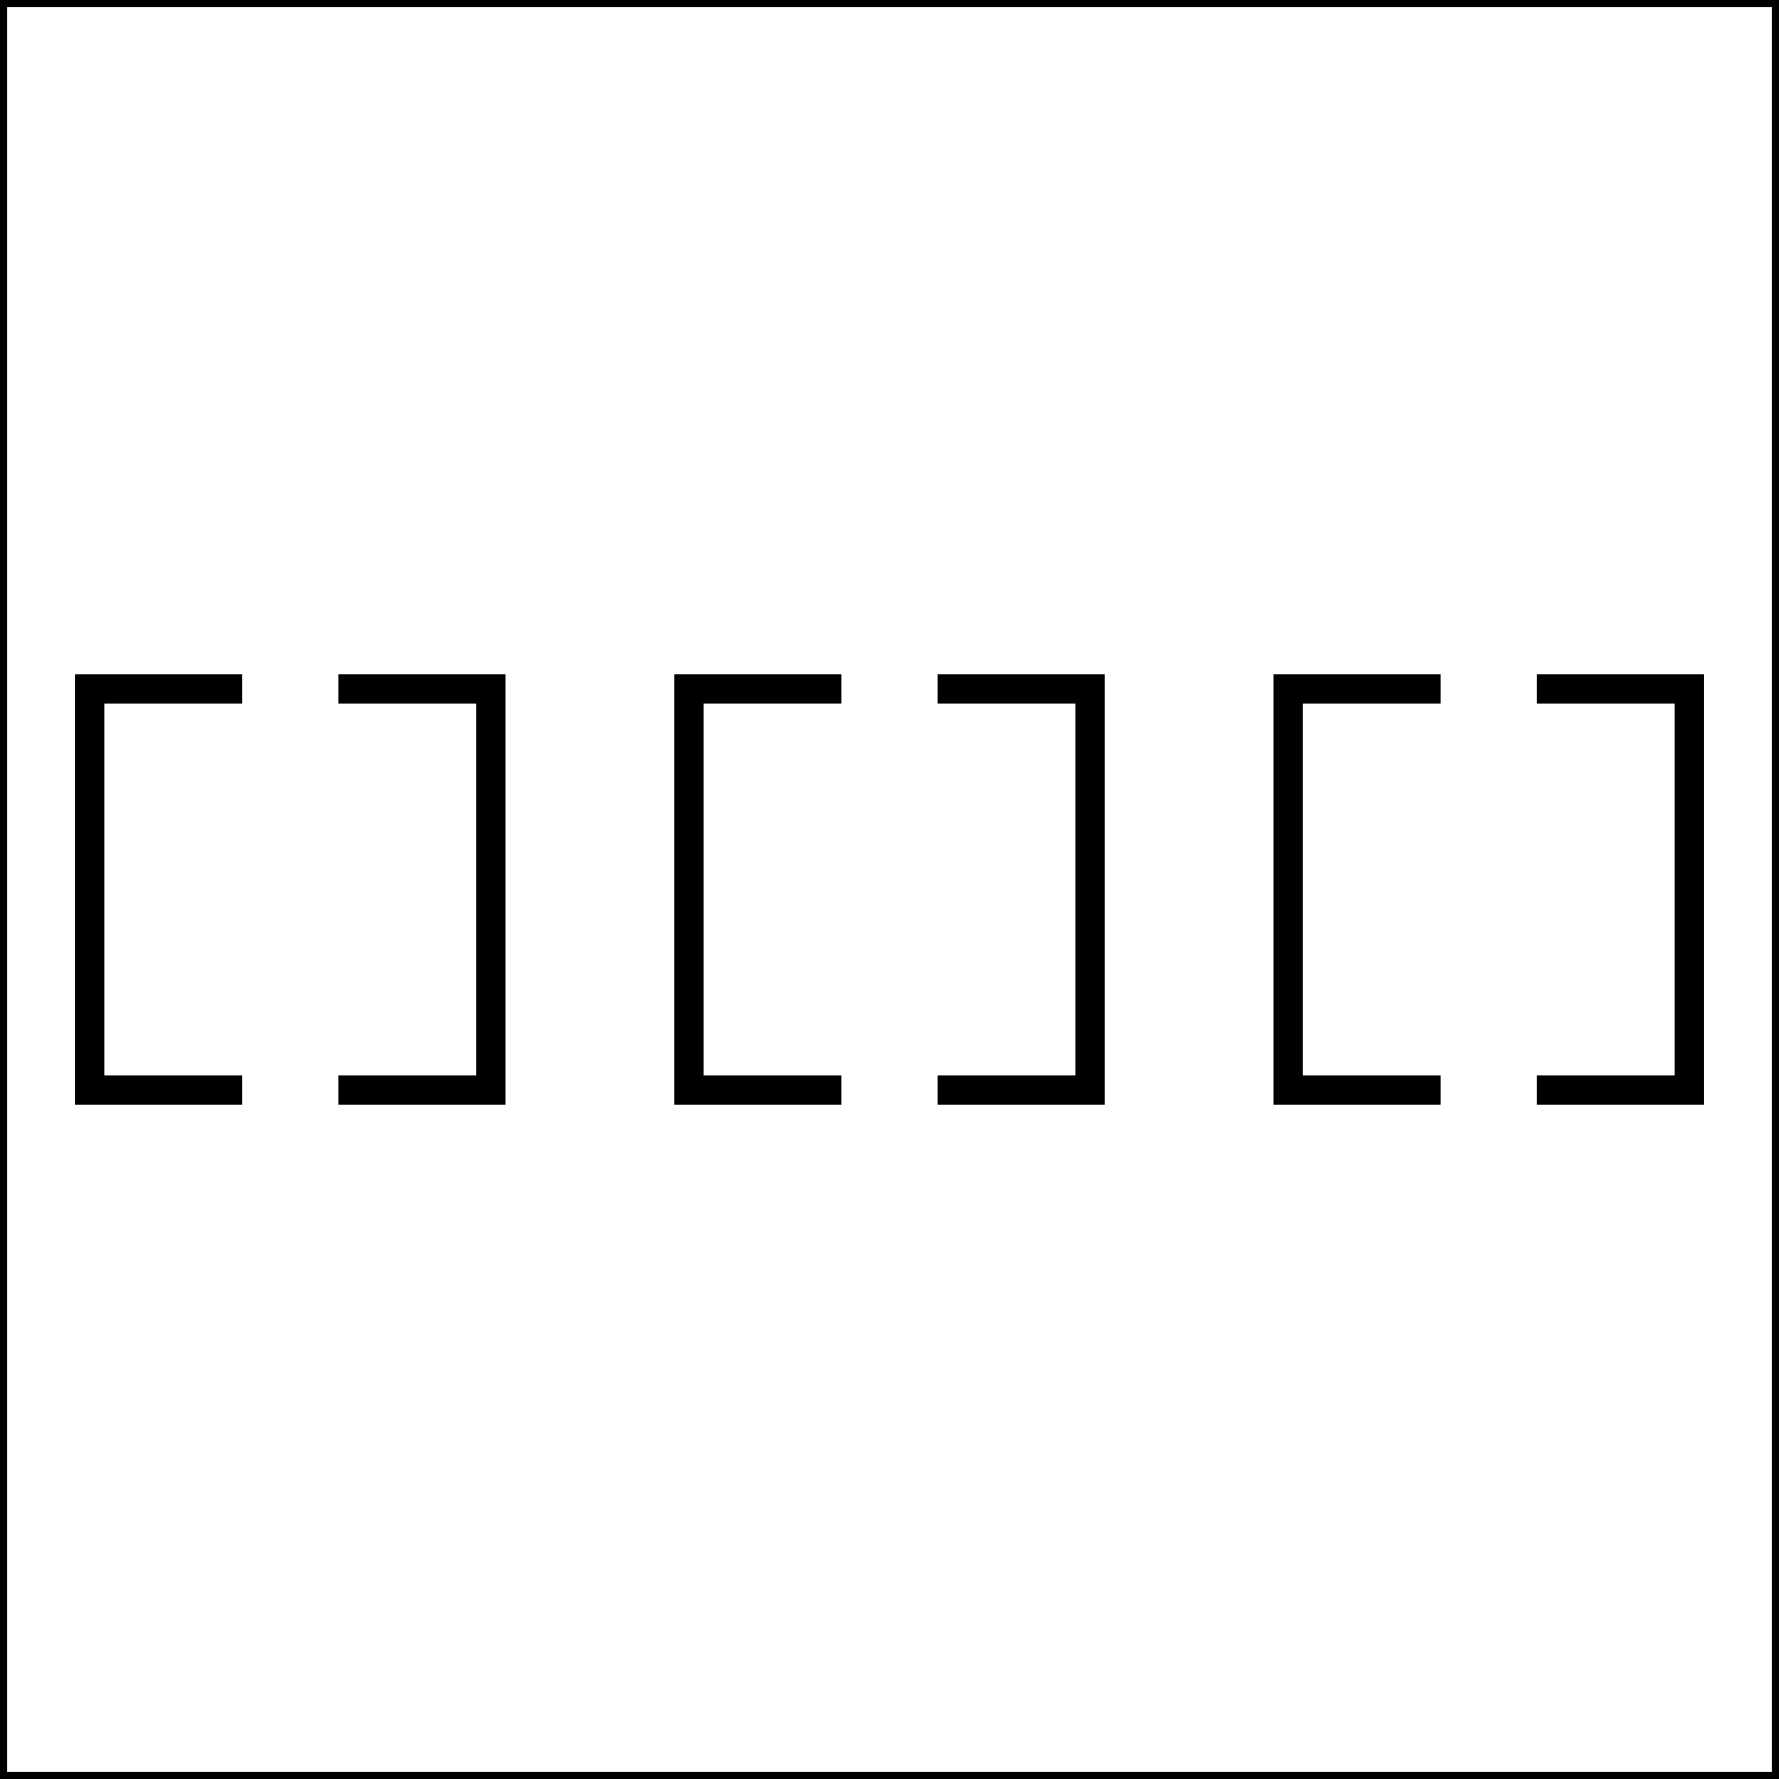
\includegraphics[width=\textwidth]{gestalt_closure}
        \caption{Closure}
        \label{fig:gestalt_closure}
    \end{subfigure}
        ~ %add desired spacing between images, e. g. ~, \quad, \qquad, \hfill etc. 
      %(or a blank line to force the subfigure onto a new line)
    \begin{subfigure}[b]{0.25\textwidth}
        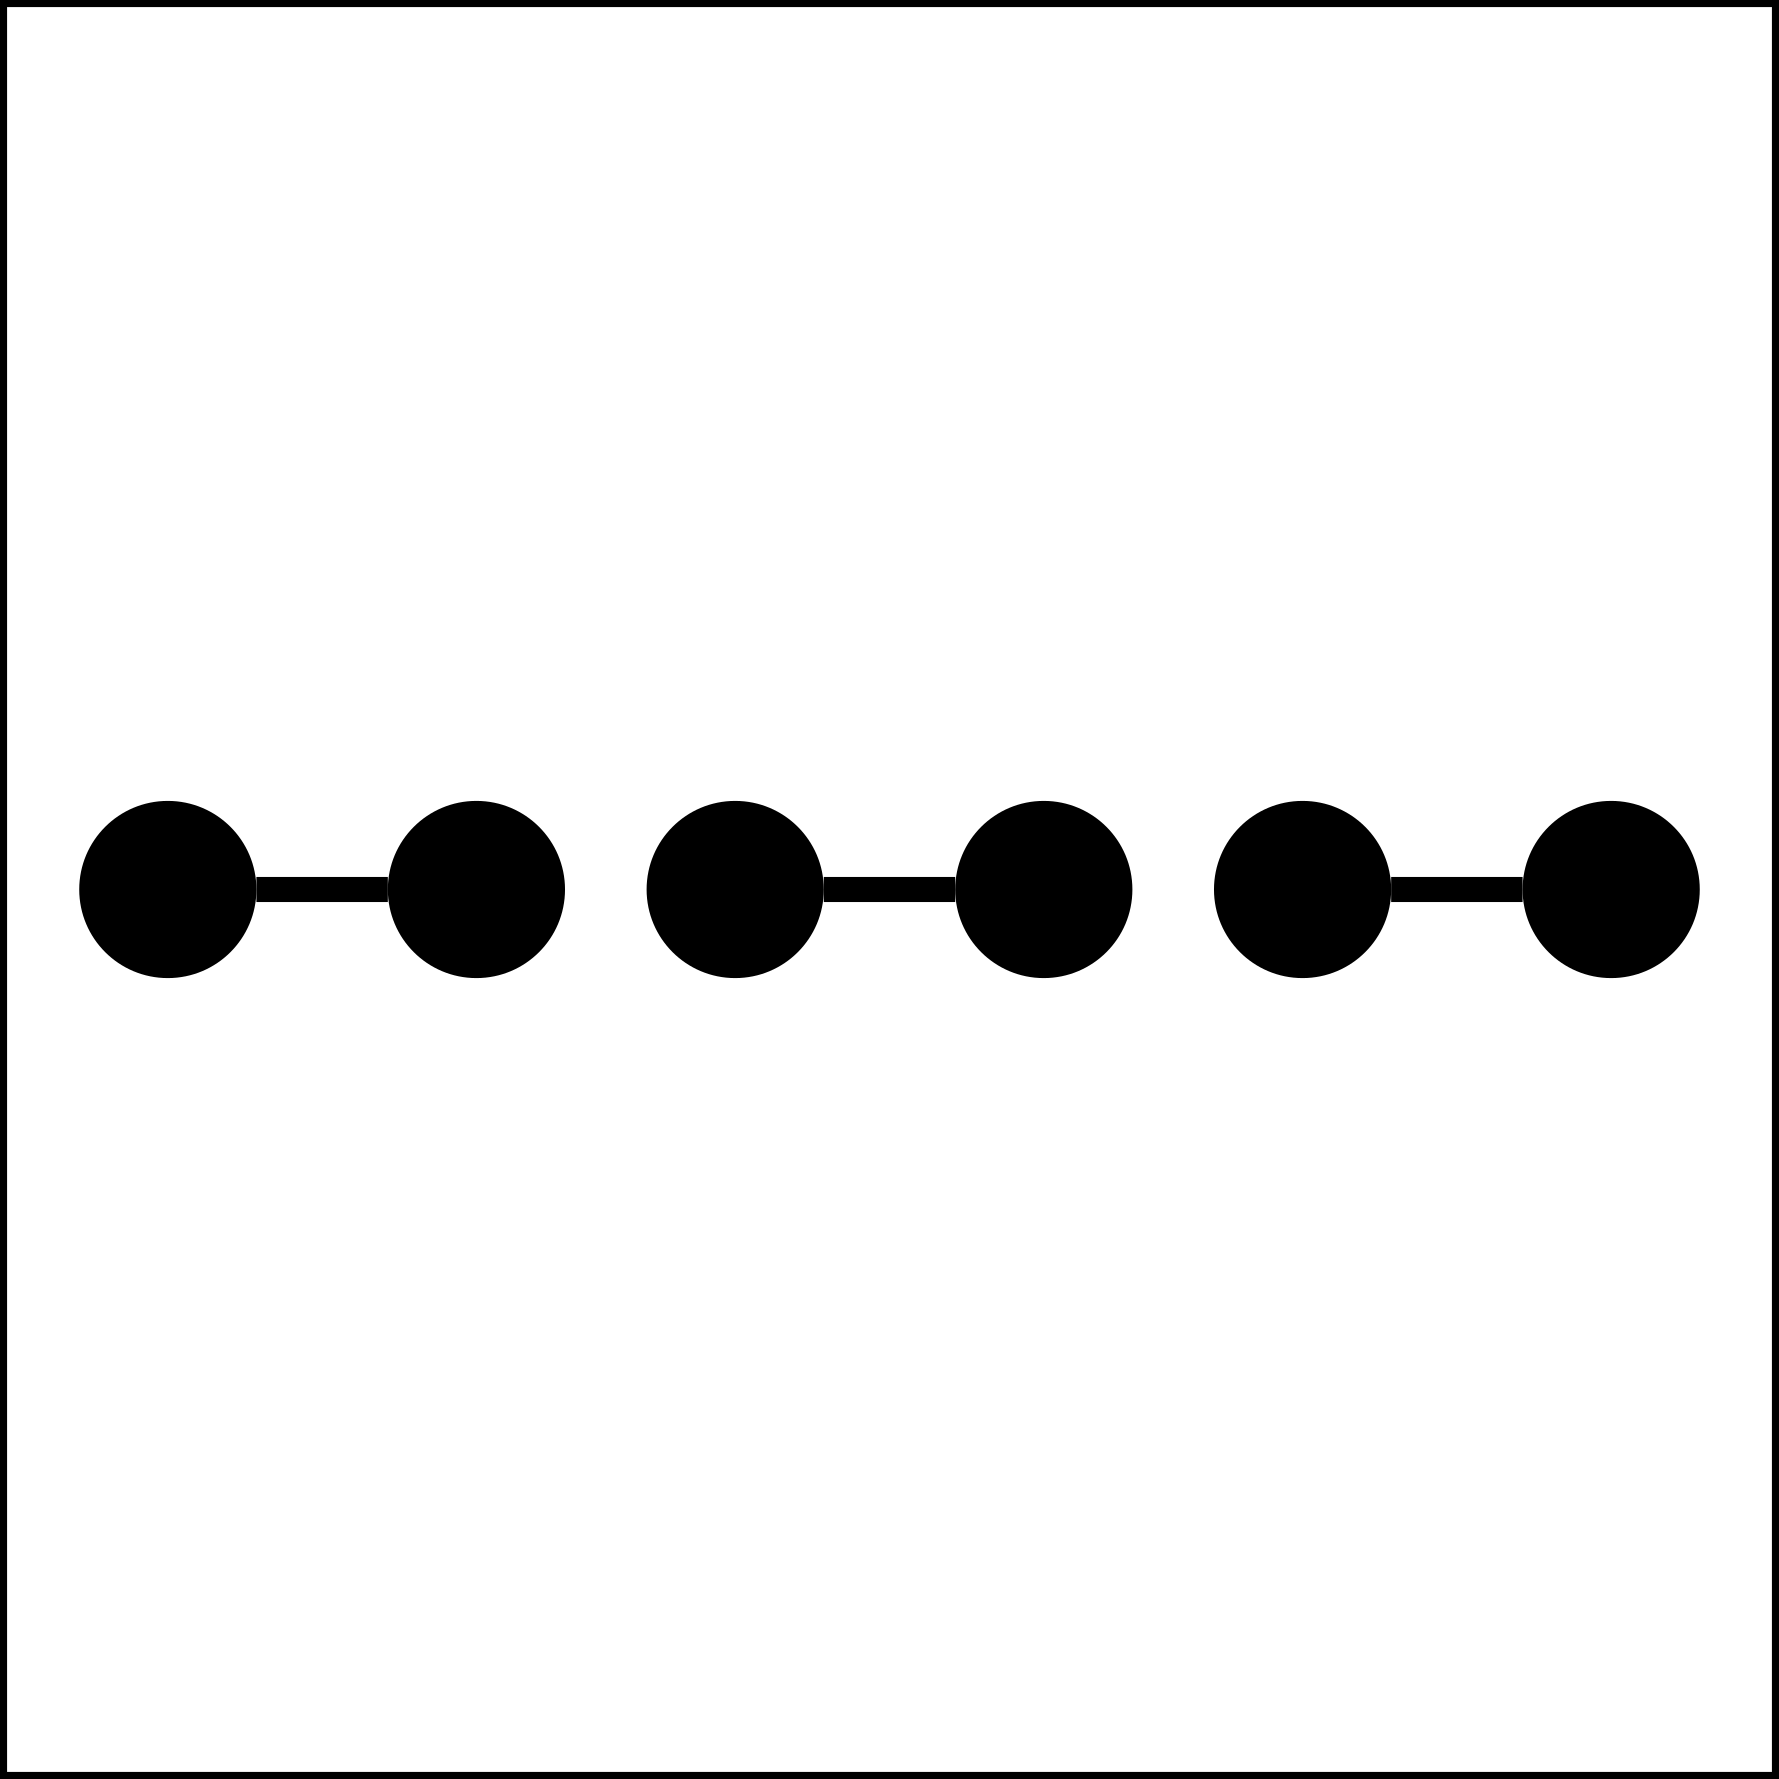
\includegraphics[width=\textwidth]{gestalt_connectedness}
        \caption{Connectedness}
        \label{fig:gestalt_connectedness}
    \end{subfigure}
    
    \caption{Graphic representation of the grouping Gestalt laws.}\label{fig:gestalt_laws}
\end{figure}

In this work, we explore the above ideas and propose a novel approach to detect a landing target in the same way humans do, imitating the human perception process. To achieve the detection, we use the intensity image contours retrieved at different scales. We obtain the most perceptual contours from this set of contours: those not generated by chance using an a contrario approach. After this procedure, we take advantage of the predefined form of the targets to propose some measures representing the grouping laws of similarity and proximity of the Gestalt. Finally, we do the decoding and correction of target identification errors using Hamming's code. The diagram shown in figure \ref{fig:target_detection_pipeline} groups the stages of our method for the perceptual detection of landing targets.

\begin{figure}[!ht]
    \centering
    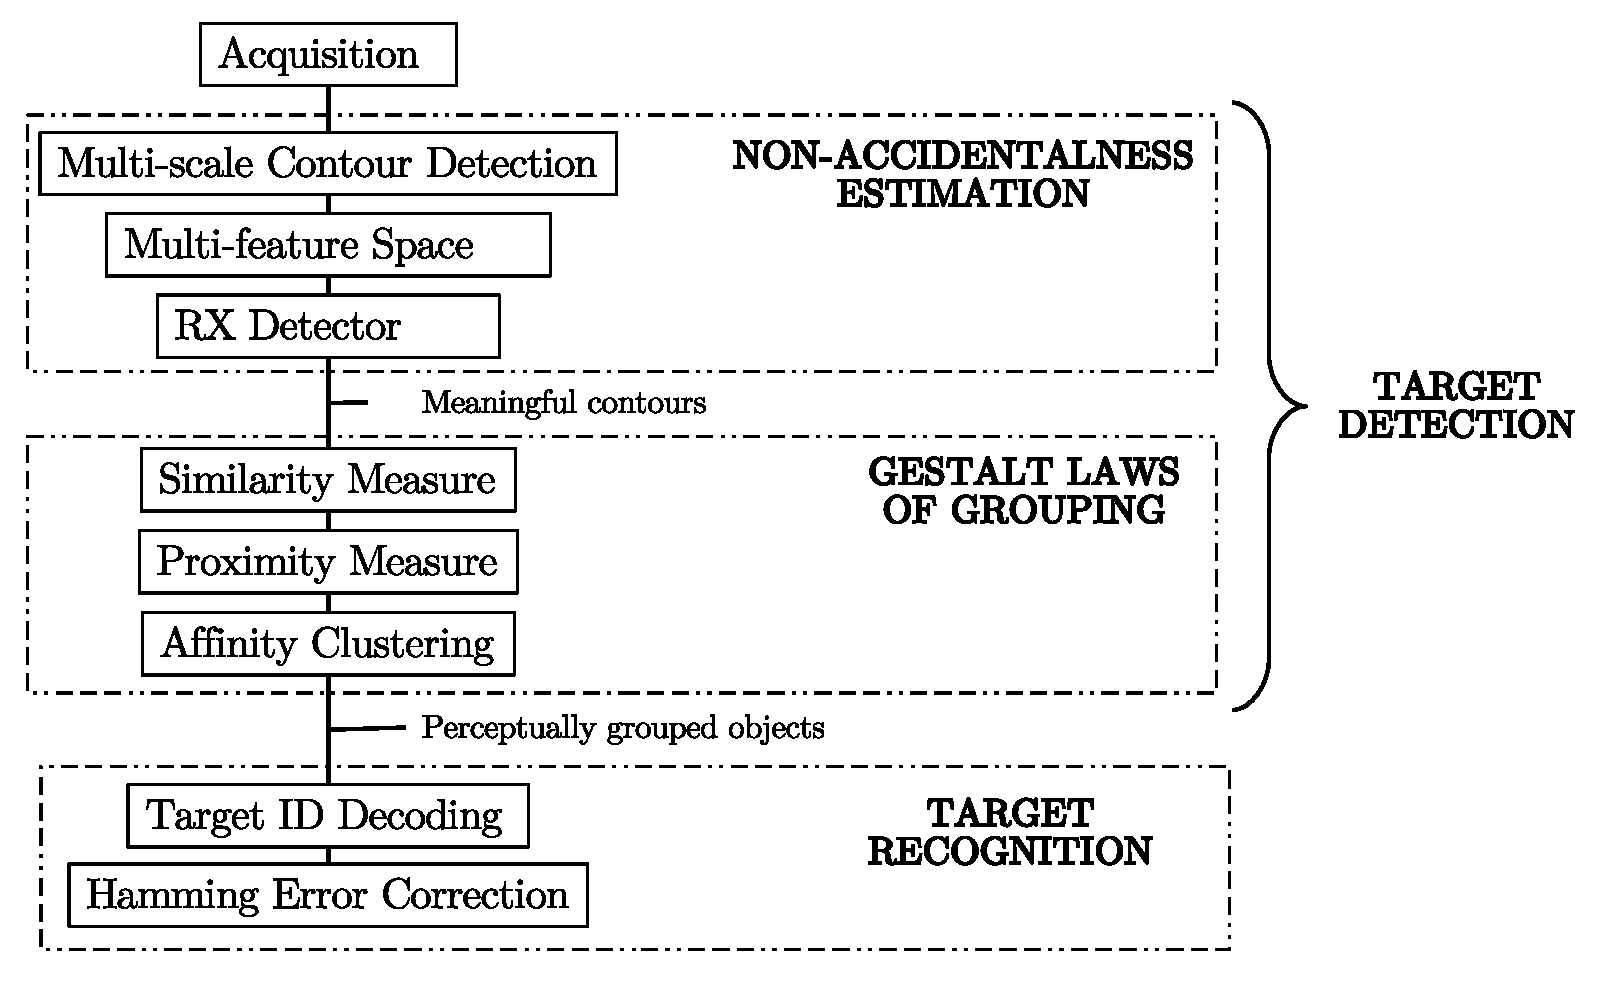
\includegraphics[width=\textwidth]{target_detection_pipeline}        
    \caption{Diagram of the phases involved in the landing target detection and recognition task.}\label{fig:target_detection_pipeline}
\end{figure}

The following sections are devoted to detailing the framework for the detection of landing targets. In section \ref{sec:hierarchical_target_detection}, we evaluate different threshold-based methods for obtaining contours in an algorithm that uses the hierarchy of contours to detect landing targets. After that, we develop our perception model in section \ref{sec:unsupervised_perception_model}. Specifically, subsection \ref{subsec:Helmholtz} describes how to retrieve image contours as meaningful primitives, and subsection \ref{subsec:Gestalt} describes how to group the contours to detect a landing target perceptually. Later, in section \ref{sec:validation_and_test}, we present the implementation of our methodology and some tests with both synthetic and real-life images. We also present some conclusions and perspectives in section \ref{sec:conclusions_landing_target}. Finally, the appendix \ref{ch:target_description} contains the description of the landing target and the strategy used for the generation and coding of information into the landing targets.


\section{Hierarchical Countours for Target Detection}\label{sec:hierarchical_target_detection}

Initially, the idea of landing targets detection is inspired by the needs of the \cite{Internest:WebPage:} company. The objective is to design a landing marker and an algorithm for its detection; all of this in the context of the UAV's autonomous precision landing task. A first approach, developed during the traineeship period of a master student \citep{BaquedanoA.:ESIEE:2017}, seeks to solve the task straightforwardly using highly studied techniques. The algorithm is based on finding the contours of a binary image generated by the threshold method proposed by \cite{Otsu:SMC:1979}. Since the landing target they suggest is composed of nested concentric circles, they heuristically use the hierarchy of the found contours to detect a landing target. Their methodology consists of discriminating the contours that are not nested through conditional evaluations at each hierarchy level. The conditions are hierarchically dependent, which means that the landing target detection is ineffective if the conditions are not strictly fulfilled.

They tested this approach; however, similarly to some other works mentioned in section \ref{sec:introduction_ch1}, the algorithm works well only under certain circumstances. The tests show that the algorithm fails in most cases because it is not able to find all the target contours, which compromises the hierarchical condition for detection. This effect generally occurs when the landing target is exposed to conditions that degrade the quality of the image. Given the nature of the aerial object detection task, factors such as the change in height and orientation of the UAV modify an object's perception, introducing disturbances such as noise, changes in lighting and contrast, deformation of objects, etc. Such image degradations complicate the operation of threshold-based methods and consequently the detection of contours. We classify the disturbances suffered by landing targets into four types: 

\begin{enumerate}
	\item Change in size w.r.t. the scene.
	\item Presence of noise.
	\item Presence of shadows.
	\item Deformation due to perspective.
\end{enumerate}
Figure \ref{fig:tar_degradations} shows a landing target affected by the disturbances mentioned above.

  
\begin{figure}[!ht]
    \centering
    \begin{subfigure}[b]{0.3\textwidth}
        \frame{
\includegraphics[width=\textwidth]{tar_noise}}
        \caption{}
        \label{fig:deg_noise}
    \end{subfigure}
        ~ %add desired spacing between images, e. g. ~, \quad, \qquad, \hfill etc. 
      %(or a blank line to force the subfigure onto a new line)
    \begin{subfigure}[b]{0.3\textwidth}
        \frame{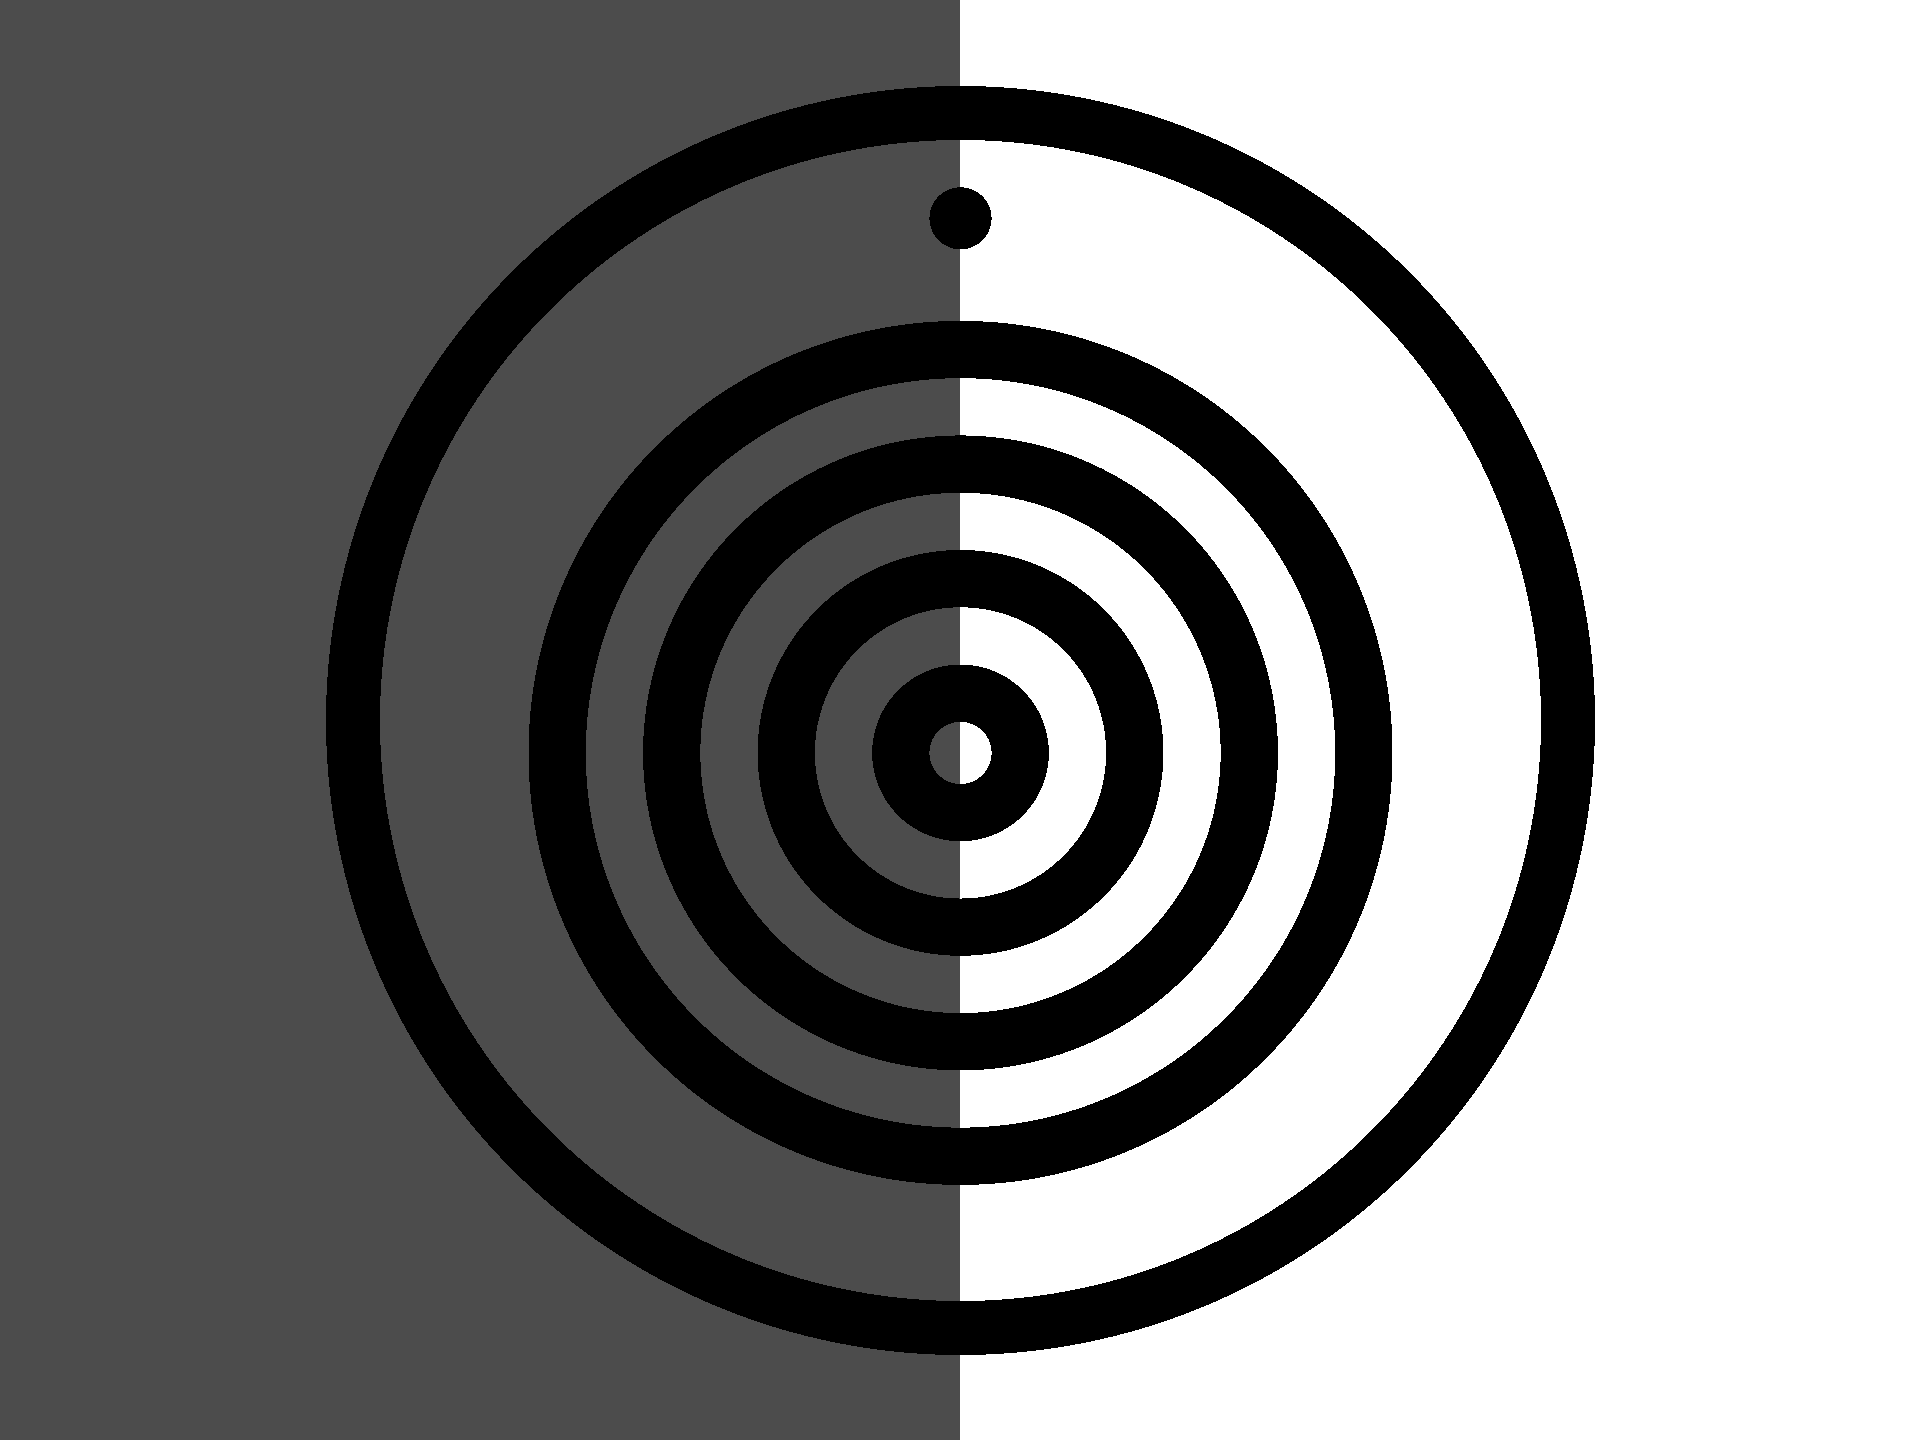
\includegraphics[width=\textwidth]{tar_shadow}}
        \caption{}
        \label{fig:deg_shadow}
    \end{subfigure}\\
        ~ %add desired spacing between images, e. g. ~, \quad, \qquad, \hfill etc. 
      %(or a blank line to force the subfigure onto a new line)
    \begin{subfigure}[b]{0.3\textwidth}
        \frame{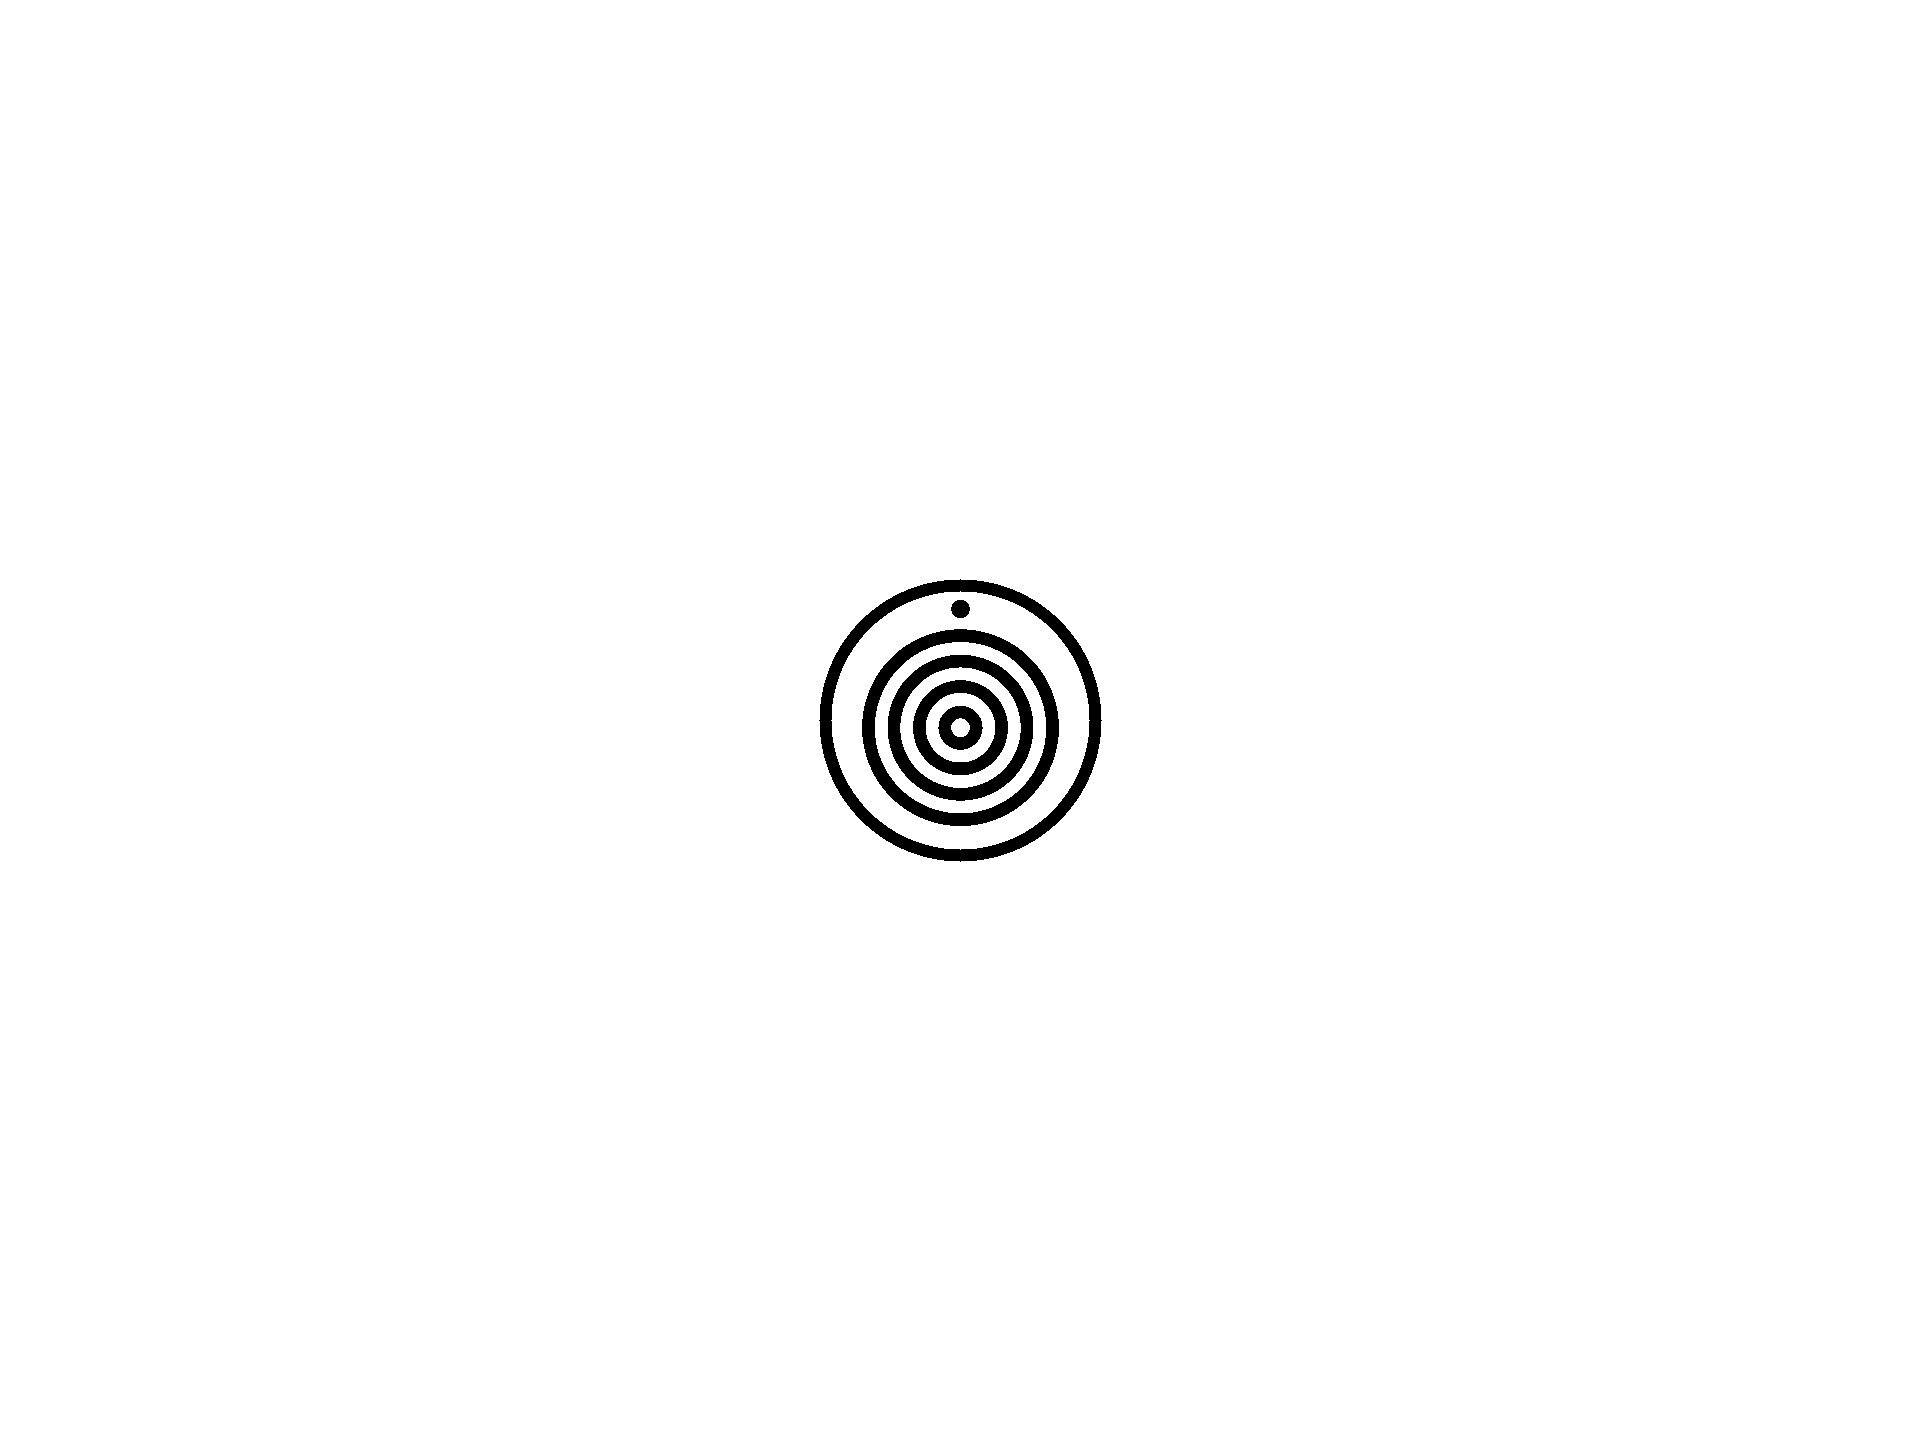
\includegraphics[width=\textwidth]{tar_resolution}}
        \caption{}
        \label{fig:deg_resolution}
    \end{subfigure}
        ~ %add desired spacing between images, e. g. ~, \quad, \qquad, \hfill etc. 
      %(or a blank line to force the subfigure onto a new line)
    \begin{subfigure}[b]{0.3\textwidth}
        \frame{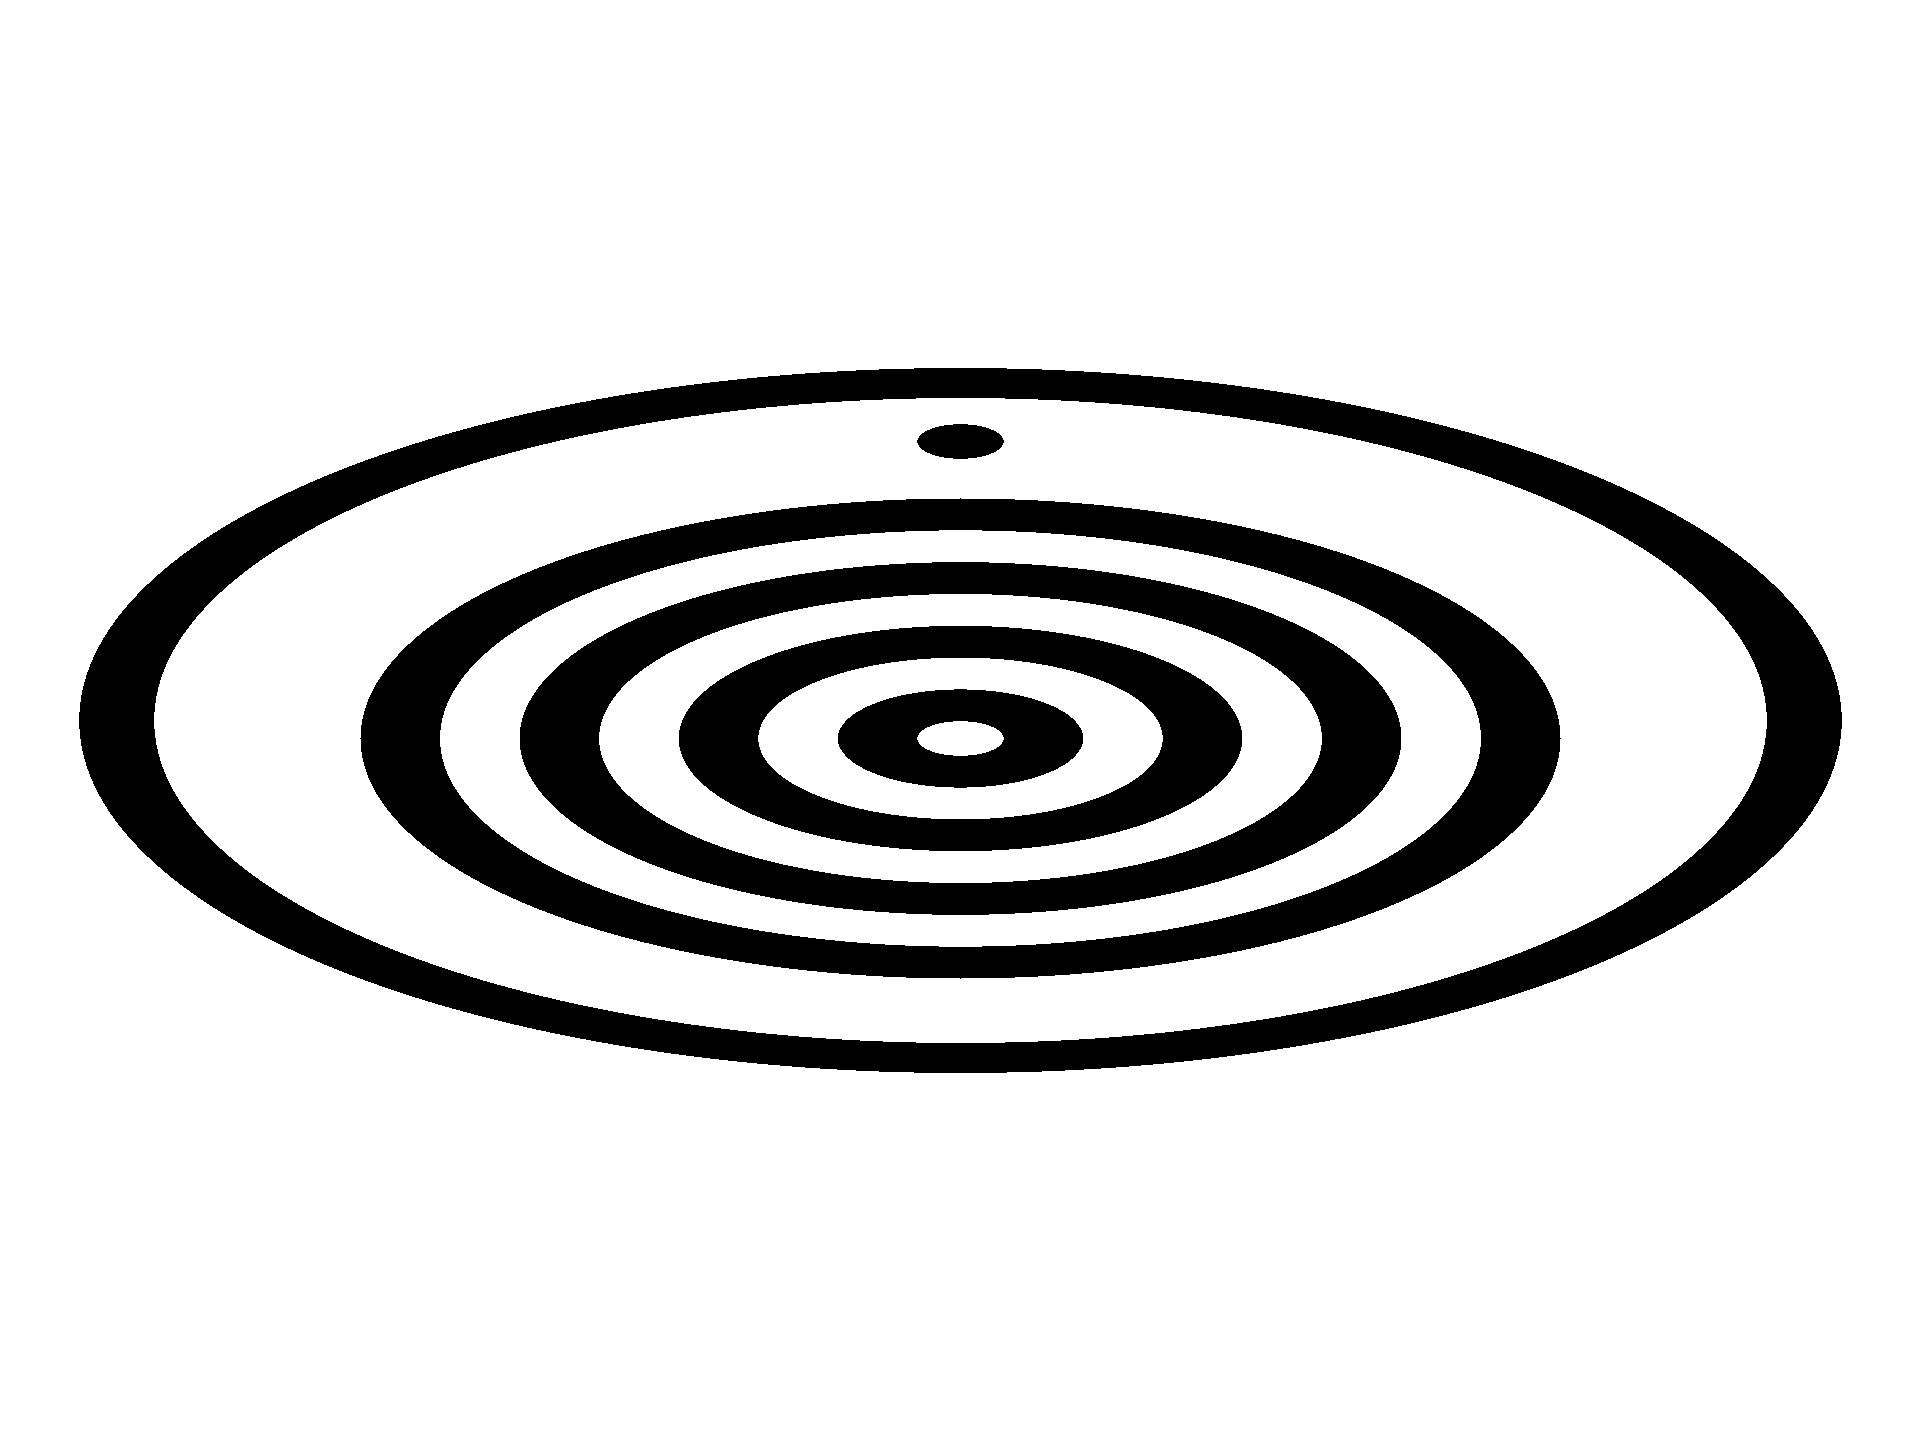
\includegraphics[width=\textwidth]{tar_deformation}}
        \caption{}
        \label{fig:deg_deformation}
    \end{subfigure}
    \caption{ Landing target degradations: \captext{(a)} Noise, \captext{(b)} Shadow, \captext{(c)} Change of size and \captext{(d)} Perspectice deformation.}\label{fig:tar_degradations}
\end{figure}


One of the main disadvantages of the hierarchy method for the landing targets detection is that its effectiveness lies with the Otsu contour detector, which does not work well in images with high contrast or severe lighting changes. However, other threshold-based methods for contour detection could better face the image degradations shown in the figure \ref{fig:tar_degradations}. Following the taxonomy for threshold-based methods proposed in \citep{Sezgin.Sankur:EI:2010}, there are clustering-based methods such as \cite{Otsu:SMC:1979} and \cite{Ridler.Calvard:TSMC:1978} edge detectors; entropy-based methods such as \cite{Yen.Chang.ea:TIP:1995} and \cite{Li.Lee:ICPR:1993} detectors; local methods such as \cite{Niblack:ImageProcc:1986} and \cite{Sauvola.Pietikainen:ICPR:2000} operators; the adaptive method proposed by \cite{Bradley.Roth:ACM:2007} and finally, the mean and Gaussian pixel distribution as spacial methods. We use these nine representative threshold-based methods to obtain a binary image, localize the image contours, and evaluate the best approach facing the image degradations shown in the figure \ref{fig:tar_degradations}.


\begin{figure}[htbp]
\centering
\begin{subfigure}[t]{\dimexpr0.15\textwidth+20pt\relax}
    \makebox[20pt]{\raisebox{30pt}{\rotatebox[origin=c]{90}{Input}}}%Input (zoom)
    \frame{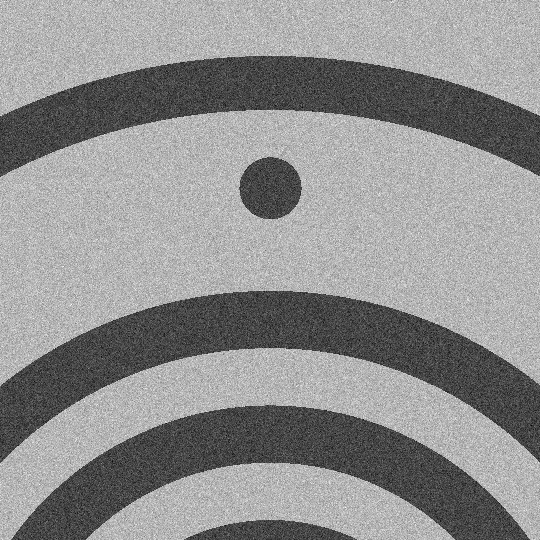
\includegraphics[width=\dimexpr\linewidth-20pt\relax]
    {tar_zoom_noise}}
    \makebox[20pt]{\raisebox{30pt}{\rotatebox[origin=c]{90}{Otsu}}}%
    \frame{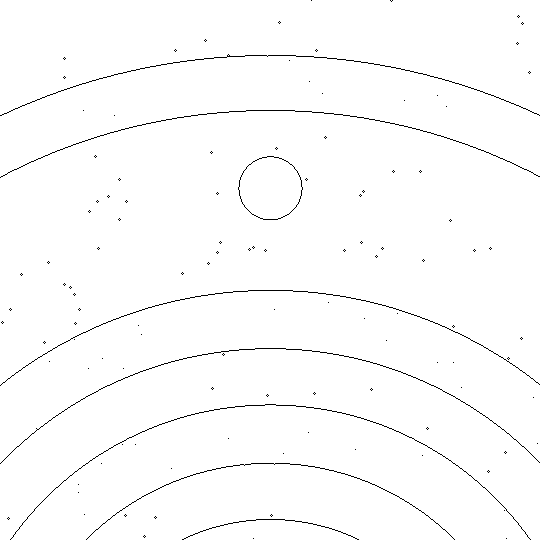
\includegraphics[width=\dimexpr\linewidth-20pt\relax]
    {Otsu_cont_noise}}
    \makebox[20pt]{\raisebox{30pt}{\rotatebox[origin=c]{90}{Riddler}}}%
    \frame{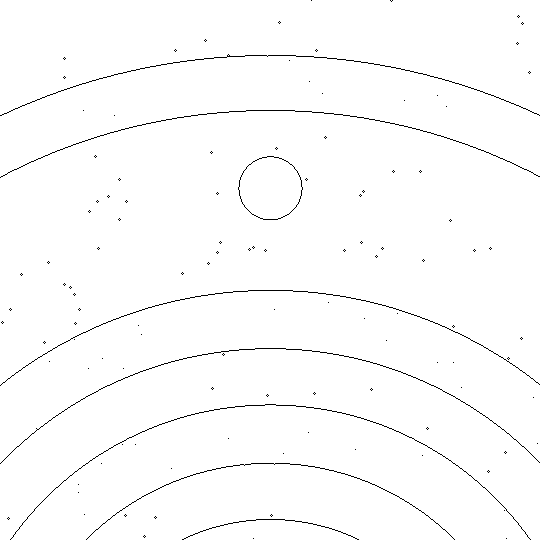
\includegraphics[width=\dimexpr\linewidth-20pt\relax]
    {Riddler_cont_noise}}
    \makebox[20pt]{\raisebox{30pt}{\rotatebox[origin=c]{90}{Yen}}}%
    \frame{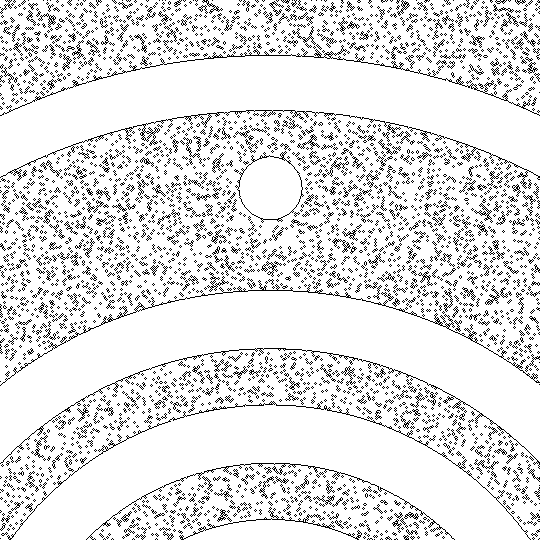
\includegraphics[width=\dimexpr\linewidth-20pt\relax]
    {Yen_cont_noise}}
    \makebox[20pt]{\raisebox{30pt}{\rotatebox[origin=c]{90}{Li}}}%
    \frame{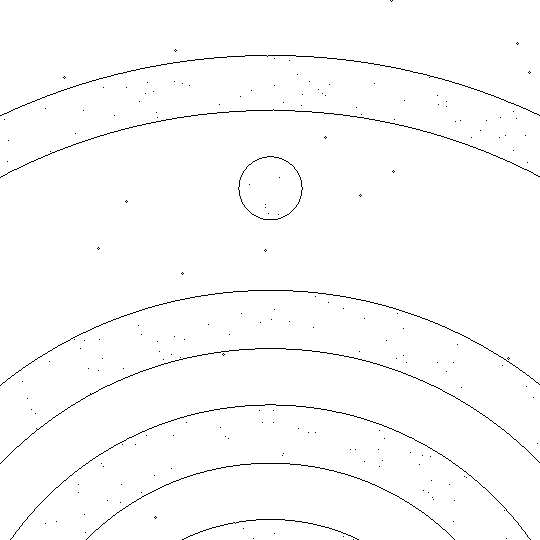
\includegraphics[width=\dimexpr\linewidth-20pt\relax]
    {Li_cont_noise}}
    \makebox[20pt]{\raisebox{30pt}{\rotatebox[origin=c]{90}{Niblack}}}%
    \frame{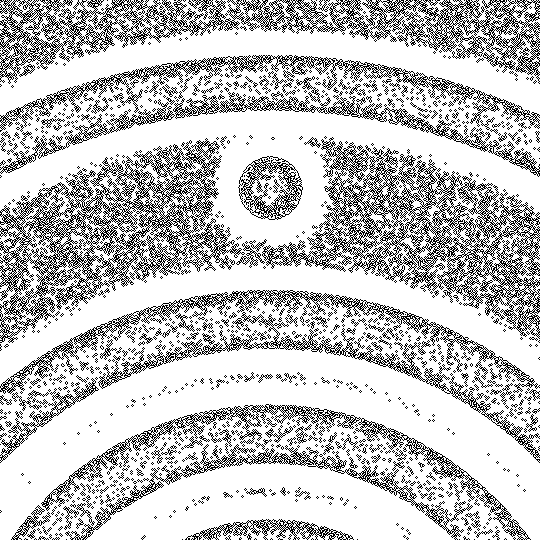
\includegraphics[width=\dimexpr\linewidth-20pt\relax]
    {Niblack_cont_noise}}
    \makebox[20pt]{\raisebox{30pt}{\rotatebox[origin=c]{90}{Sauvola}}}%
    \frame{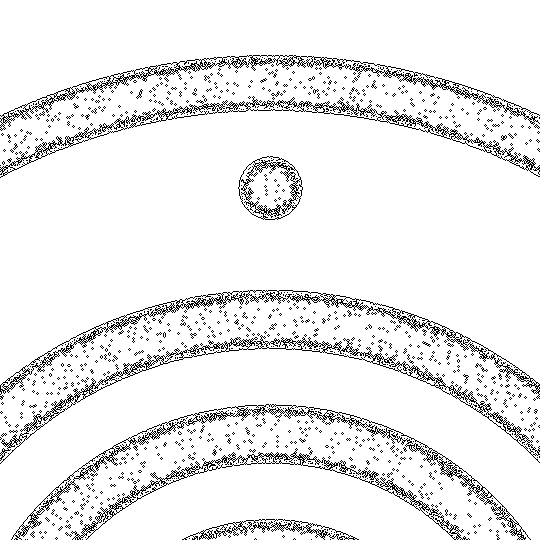
\includegraphics[width=\dimexpr\linewidth-20pt\relax]
    {Sauvola_cont_noise}}
    \makebox[20pt]{\raisebox{30pt}{\rotatebox[origin=c]{90}{Bradley}}}%
    \frame{
\includegraphics[width=\dimexpr\linewidth-20pt\relax]
    {Bradley_cont_noise}}
    \makebox[20pt]{\raisebox{30pt}{\rotatebox[origin=c]{90}{Gauss}}}%
    \frame{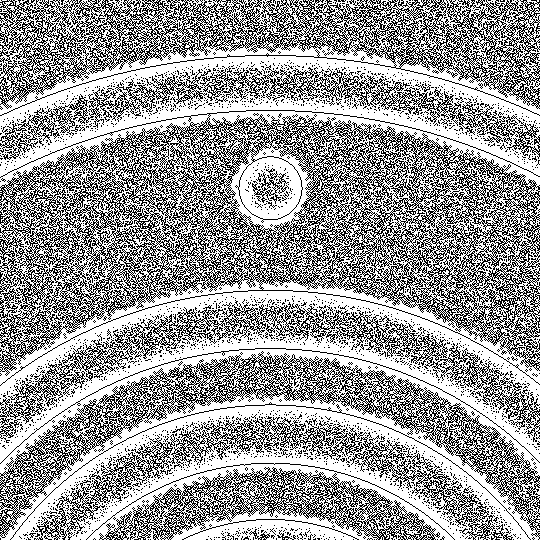
\includegraphics[width=\dimexpr\linewidth-20pt\relax]
    {Gauss_cont_noise}}
    \makebox[20pt]{\raisebox{30pt}{\rotatebox[origin=c]{90}{Mean}}}%
    \frame{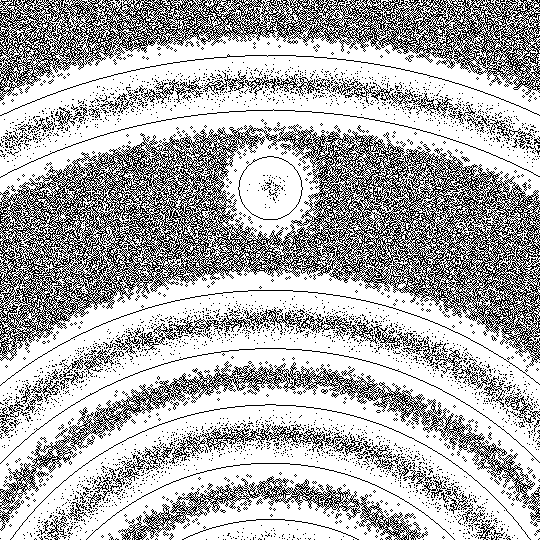
\includegraphics[width=\dimexpr\linewidth-20pt\relax]
    {Mean_cont_noise}}
    \caption{} 
\end{subfigure}\qquad
\begin{subfigure}[t]{0.15\textwidth}
    \frame{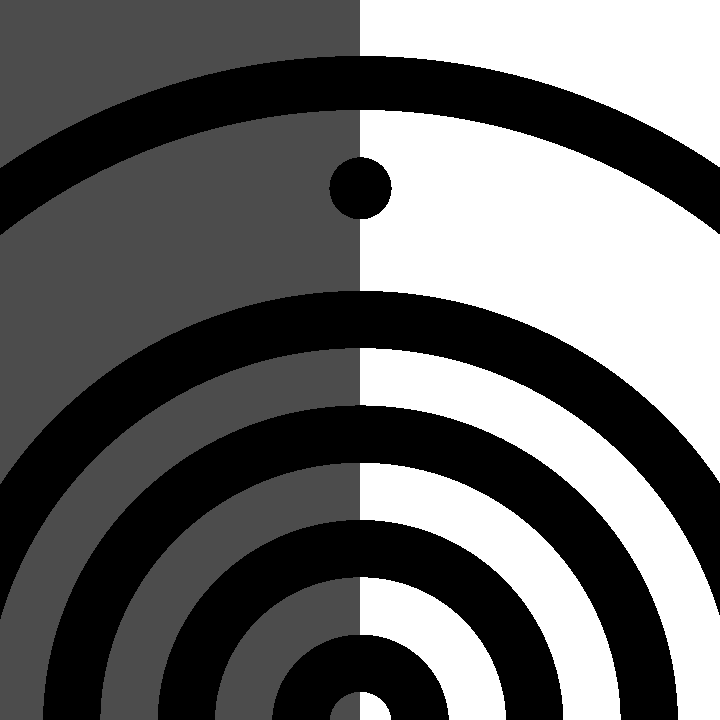
\includegraphics[width=\textwidth]
    {tar_zoom_shadow}}
    \frame{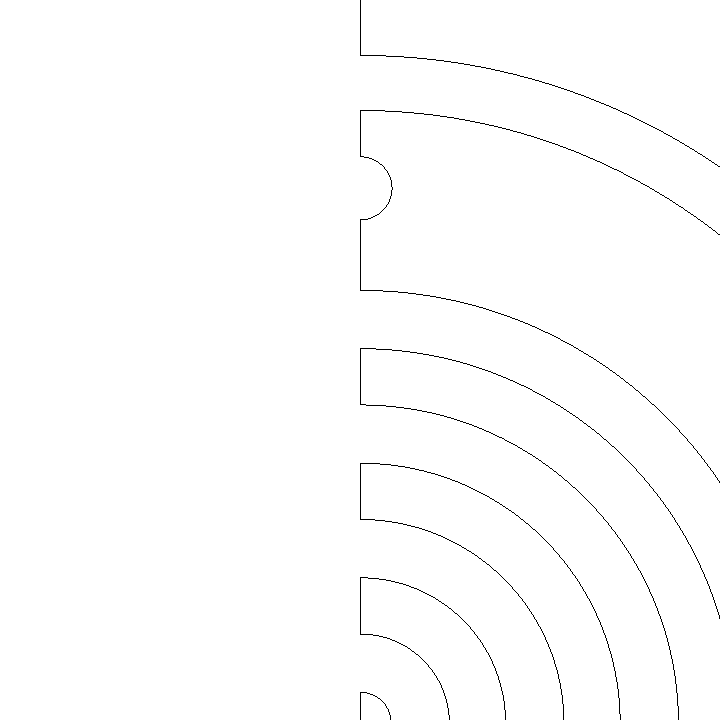
\includegraphics[width=\textwidth]
    {Otsu_cont_shadow}}
    \frame{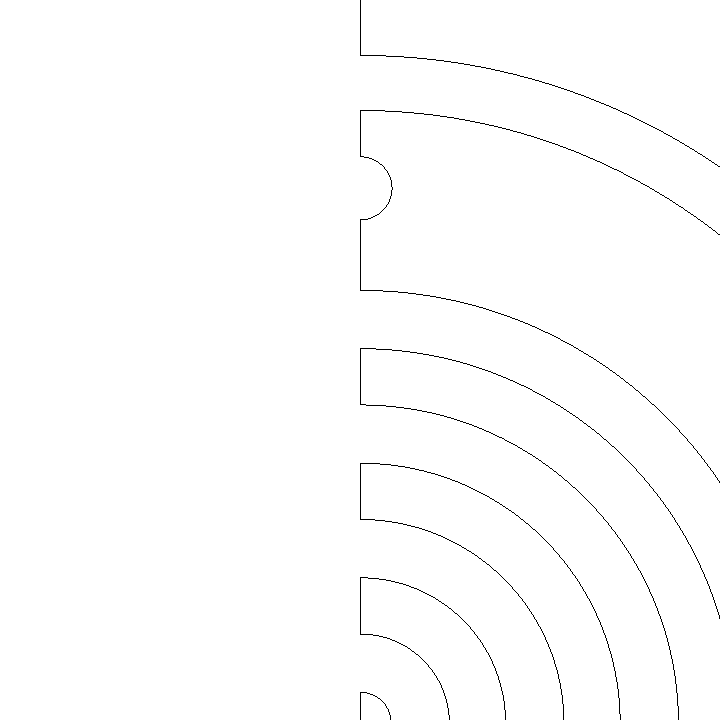
\includegraphics[width=\textwidth]
    {Riddler_cont_shadow}}
    \frame{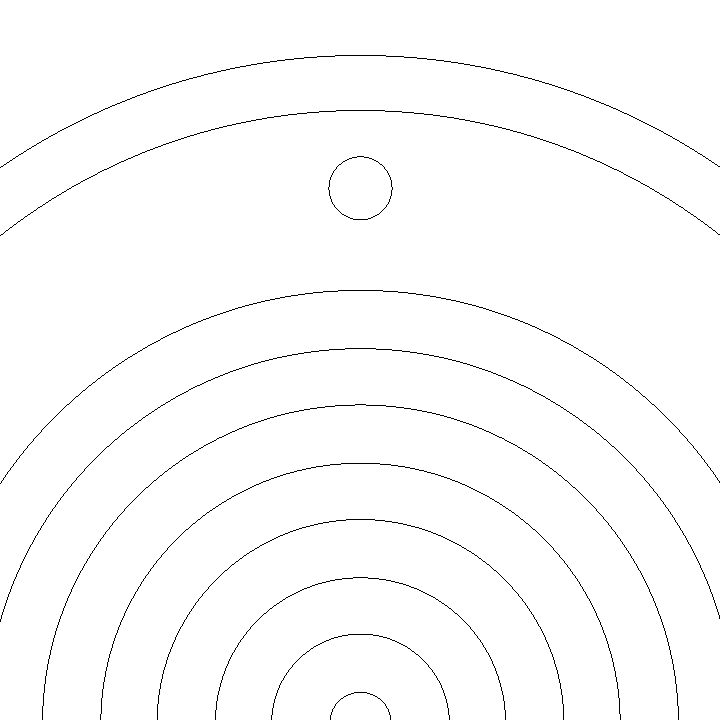
\includegraphics[width=\textwidth]
    {Yen_cont_shadow}}
    \frame{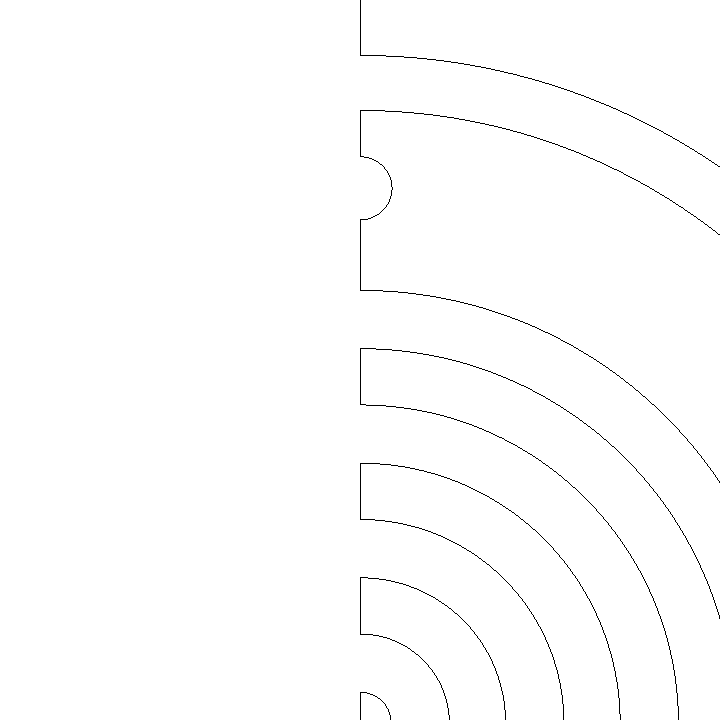
\includegraphics[width=\textwidth]
    {Li_cont_shadow}}
    \frame{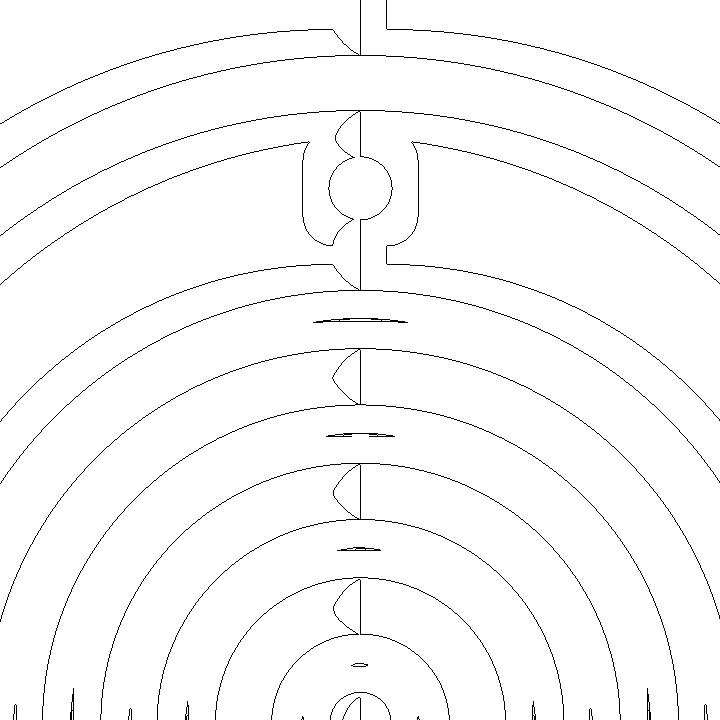
\includegraphics[width=\textwidth]
    {Niblack_cont_shadow}}
    \frame{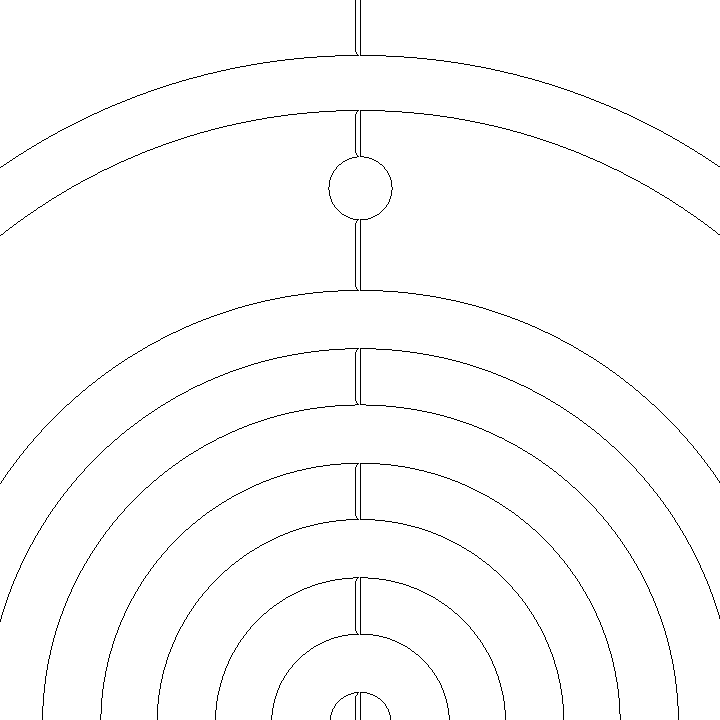
\includegraphics[width=\textwidth]
    {Sauvola_cont_shadow}}
    \frame{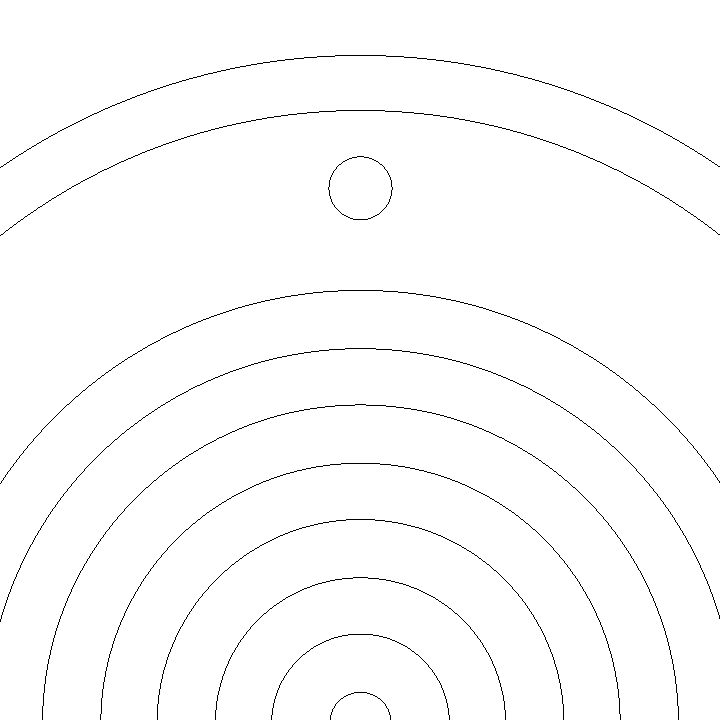
\includegraphics[width=\textwidth]
    {Bradley_cont_shadow}}
    \frame{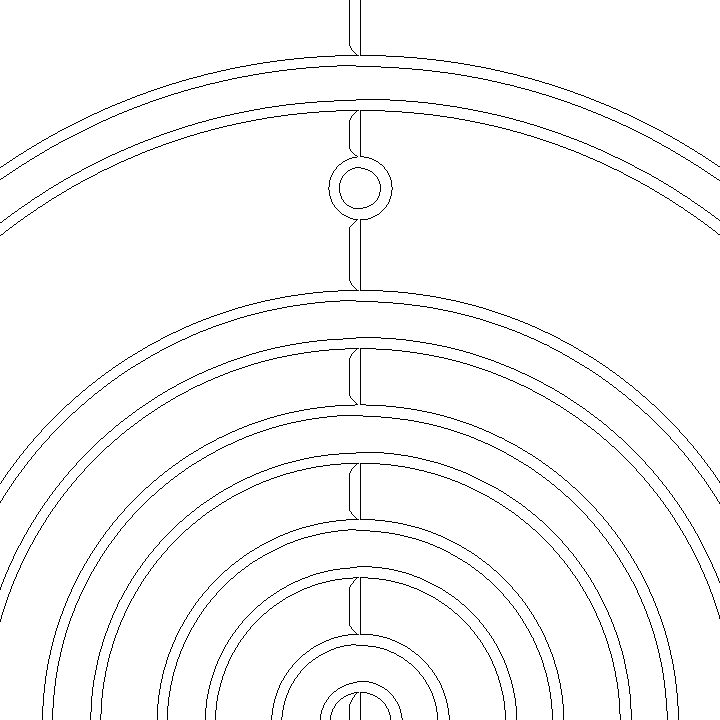
\includegraphics[width=\textwidth]
    {Gauss_cont_shadow}}
    \frame{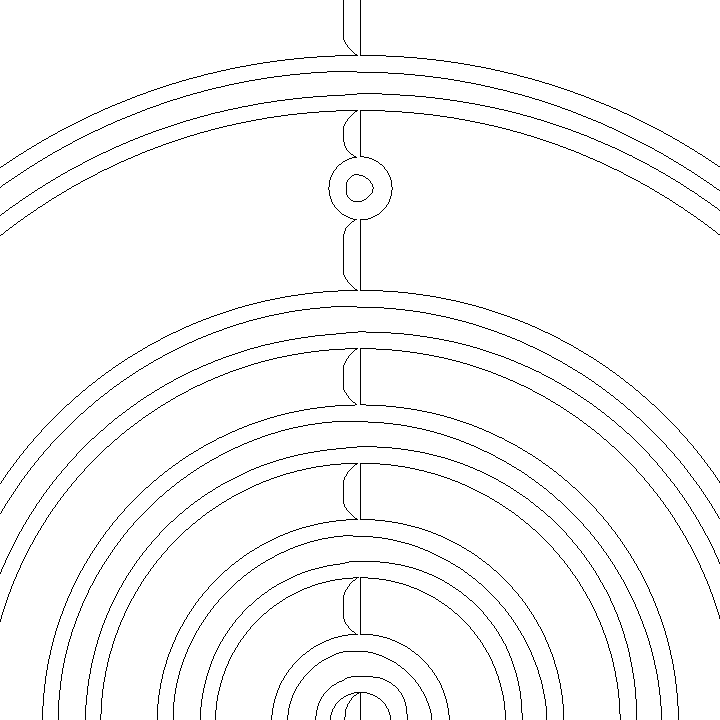
\includegraphics[width=\textwidth]
    {Mean_cont_shadow}}
    \caption{} 
\end{subfigure}\qquad
\begin{subfigure}[t]{0.15\textwidth}
    \frame{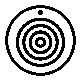
\includegraphics[width=\textwidth]
    {tar_zoom_resolution}}
    \frame{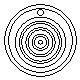
\includegraphics[width=\textwidth]
    {Otsu_cont_resolution}}
    \frame{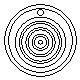
\includegraphics[width=\textwidth]
    {Riddler_cont_resolution}}
    \frame{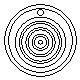
\includegraphics[width=\textwidth]
    {Yen_cont_resolution}}
    \frame{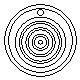
\includegraphics[width=\textwidth]
    {Li_cont_resolution}}
    \frame{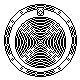
\includegraphics[width=\textwidth]
    {Niblack_cont_resolution}}
    \frame{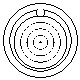
\includegraphics[width=\textwidth]
    {Sauvola_cont_resolution}}
    \frame{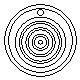
\includegraphics[width=\textwidth]
    {Bradley_cont_resolution}}
    \frame{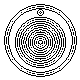
\includegraphics[width=\textwidth]
    {Gauss_cont_resolution}}
    \frame{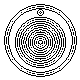
\includegraphics[width=\textwidth]
    {Mean_cont_resolution}}
    \caption{} 
\end{subfigure}\qquad
\begin{subfigure}[t]{0.15\textwidth}
    \frame{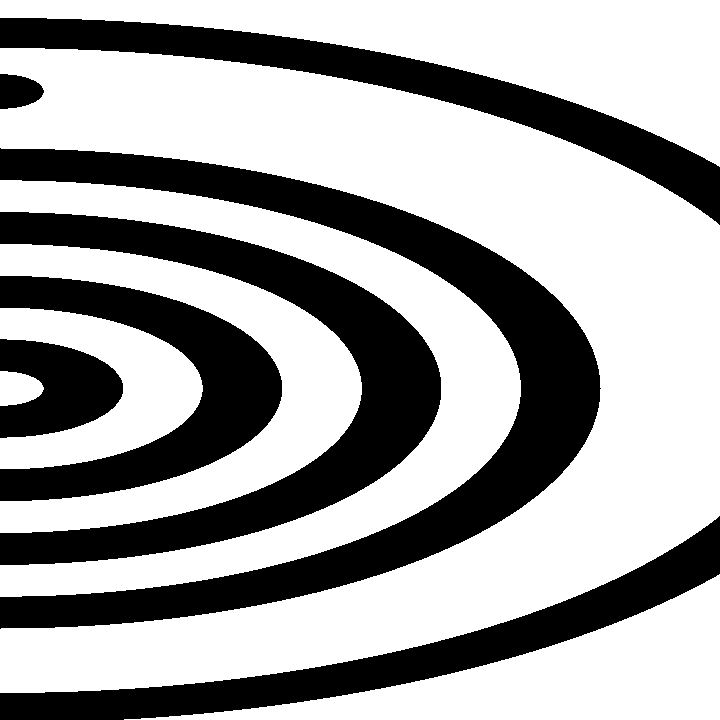
\includegraphics[width=\textwidth]
    {tar_zoom_deformation}}
    \frame{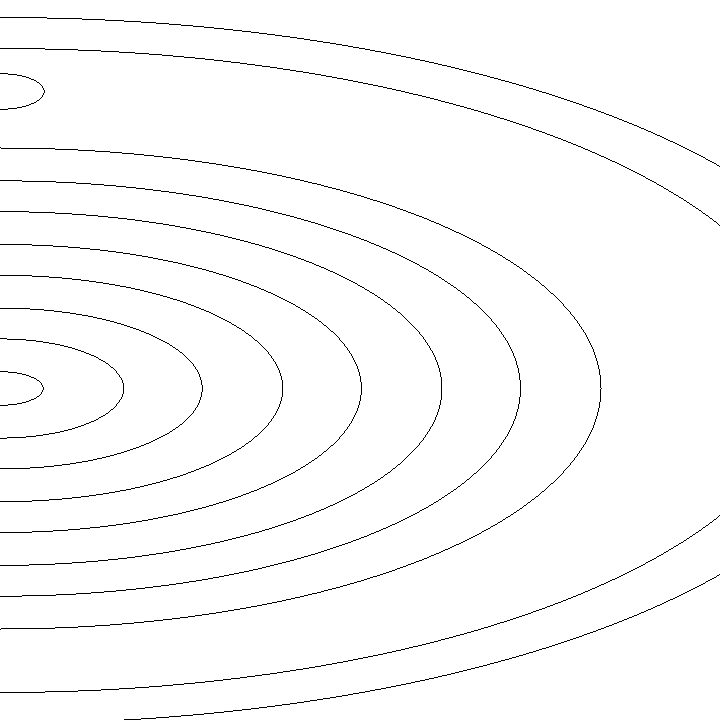
\includegraphics[width=\textwidth]
    {Otsu_cont_deformation}}
    \frame{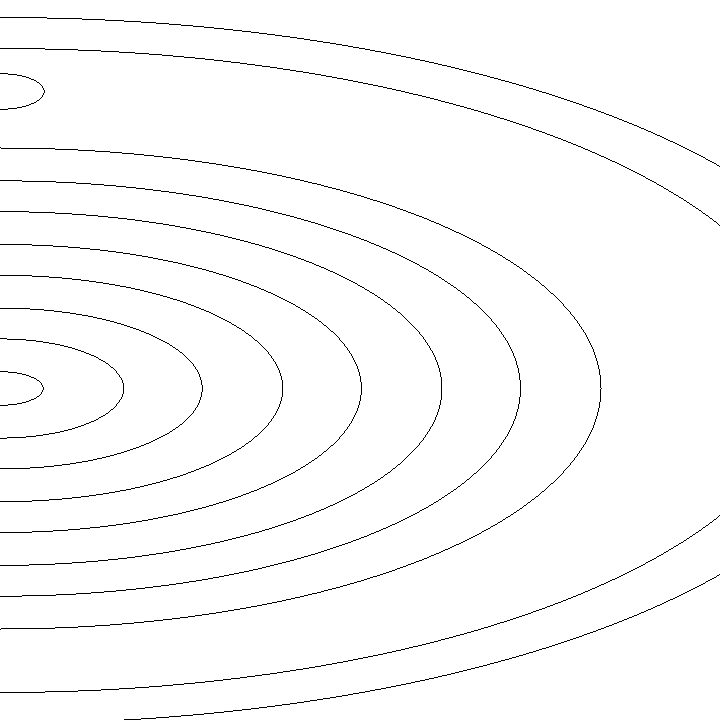
\includegraphics[width=\textwidth]
    {Riddler_cont_deformation}}
    \frame{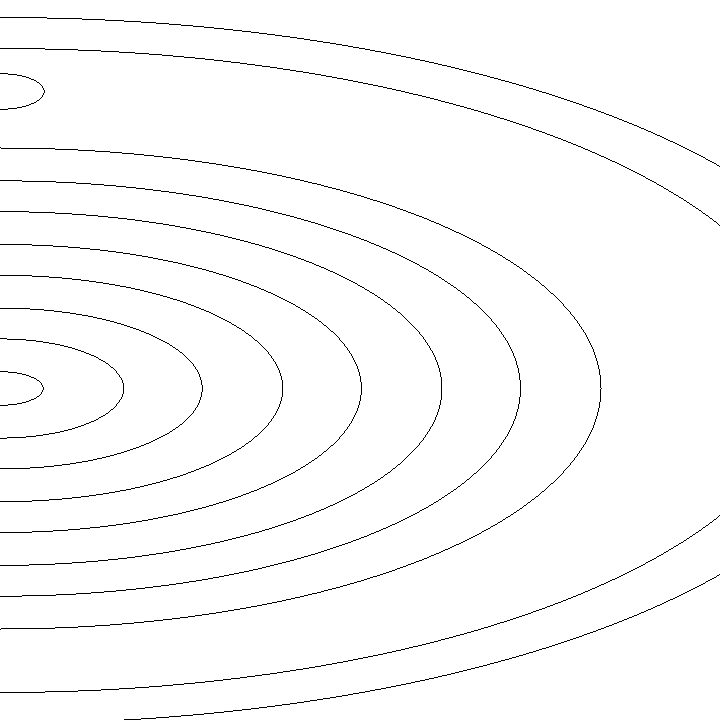
\includegraphics[width=\textwidth]
    {Yen_cont_deformation}}
    \frame{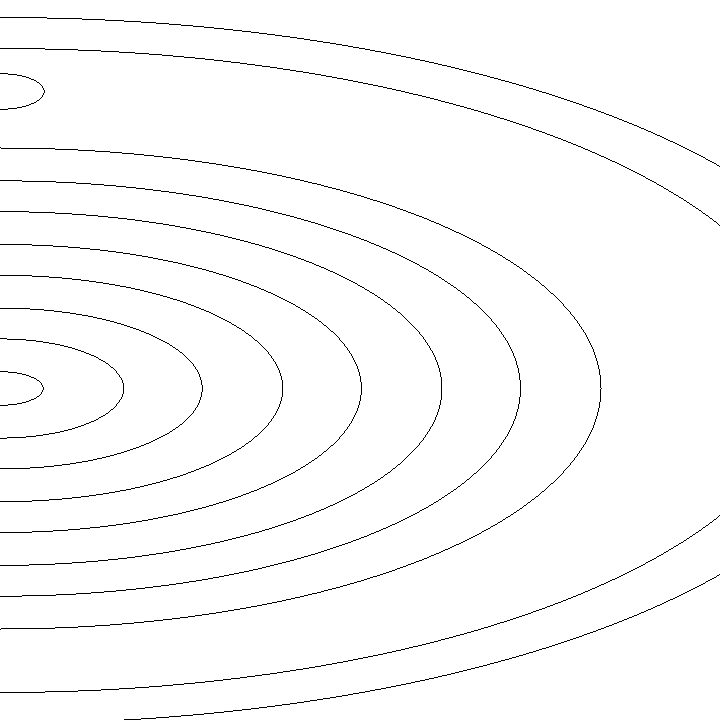
\includegraphics[width=\textwidth]
    {Li_cont_deformation}}
    \frame{\includegraphics[width=\textwidth]
    {Niblack_cont_deformation}}
    \frame{\includegraphics[width=\textwidth]
    {Sauvola_cont_deformation}}
    \frame{\includegraphics[width=\textwidth]
    {Bradley_cont_deformation}}
    \frame{\includegraphics[width=\textwidth]
    {Gauss_cont_deformation}}
    \frame{\includegraphics[width=\textwidth]
    {Mean_cont_deformation}}
    \caption{}  
\end{subfigure}
\caption{Contours obtained with the threshold-based methods applied on synthetic undergoing various degradations likely to occur in real-life conditions: \captext{(a)} Presence of noise, \captext{(b)} Presence of shadows, \captext{(c)} Change of scale, and \captext{(d)} Deformation degradations.}\label{fig:thr_synth_comparison}
\end{figure}

The contours obtained applying each threshold-based method are depicted in figure \ref{fig:thr_synth_comparison}. In this figure, we can see that the result is better or worse depending on the situation. For example, we can see that the Otsu, Riddler, Yen and Li methods react appropriately to the target scale change, but none of these four methods except the Yen operator work correctly in the presence of shadows. This results from comparing four methods under two disturbances; however, out of the nine methods, none works correctly for all perturbations.

\subsection{Threshold-based Method's Evaluation}
We run the hierarchical algorithm proposed in \citep{BaquedanoA.:ESIEE:2017} on a database of synthetic images. The database contains the sixteen different landing targets perturbed by the image degradations of figure \ref{fig:tar_degradations}. The noise degradation is simulated by adding Gaussian noise with a mean of zero and a standard deviation variable from 0.02 to 0.2, where 0.02 is the minimum noise addition. The shadow perturbation is simulated shading the left-half of the image; the variation of the shadow is done between 0 and 1, where 0 indicates a darker left-half image. The last two degradations are related to the perspective and distance of the viewer (the camera). First, we change the size of the landing target by scaling forming circles on a $640\times480$p image. The range of the scale is from 0 to 1, where 1 indicates the real scale. Lastly, we consider that the circular target behaves like an ellipse when it is not seen from the center's perpendicular axis to achieve the perspective degradation. Therefore, we deform the target synthetically by augmenting the proportion of one axis (major and minor) of the ellipse in an interval between 1 and 2, where 2 indicates the maximum deformation. 

For the test of the different contour detectors, we apply the maximum value of each degradation. We use the F1-score as a metric to evaluate each threshold-based method's accuracy under the various degradations.
\begin{equation}\label{eq:f1_score}
    \text{F1-score} = \frac{2 \times \text{precision}\times\text{recall}}{\text{precision} + \text{recall}}
\end{equation}

This metric can be interpreted as a weighted harmonic mean of the precision and recall. The precision is the ratio $tp / (tp + fp)$ and the recall is the ratio $tp / (tp + fn)$, where tp is the number of true positives, $fp$ the number of false positives, and $fn$ is the number of false negatives. The F1-score reaches its best value at 1 and its worst score at 0. Figure \ref{fig:degradations_graphs} shows the performance of all nine detectors on each disturbance separately in the form of bar plots. The graphs show the F1-score of the hierarchical detection algorithm without the Hamming error-correction (gray bars) and with the use of the Hamming error-correction (black bars) described in appendix \ref{ch:target_description}.

\begin{figure}[!ht]
    \centering
    \begin{subfigure}[b]{0.4\textwidth}
        \includegraphics[width=\textwidth]{noise_comparison}
        \caption{}
        \label{fig:noise_graph}
    \end{subfigure}
        ~ %add desired spacing between images, e. g. ~, \quad, \qquad, \hfill etc. 
      %(or a blank line to force the subfigure onto a new line)
    \begin{subfigure}[b]{0.4\textwidth}
        \includegraphics[width=\textwidth]{shade_comparison}
        \caption{}
        \label{fig:shadow_graph}
    \end{subfigure}\\
        ~ %add desired spacing between images, e. g. ~, \quad, \qquad, \hfill etc. 
      %(or a blank line to force the subfigure onto a new line)
    \begin{subfigure}[b]{0.4\textwidth}
        \includegraphics[width=\textwidth]{resolution_comparison}
        \caption{}
        \label{fig:resolution_graph}
    \end{subfigure}
        ~ %add desired spacing between images, e. g. ~, \quad, \qquad, \hfill etc. 
      %(or a blank line to force the subfigure onto a new line)
    \begin{subfigure}[b]{0.4\textwidth}
        \includegraphics[width=\textwidth]{ellipse_comparison}
        \caption{}
        \label{fig:deformation_graph}
    \end{subfigure}
    \caption{F1-score bar graphs: \captext{(a)} Noise, \captext{(b)} Shadow, \captext{(c)} Change of size and \captext{(d)} Perspectice deformation}\label{fig:degradations_graphs}
\end{figure}

Although the experiments use the highest target deformation values, they do not consider combining two or more degradations, which is closer to reality. Figure \ref{fig:input_image} shows one of our targets (target ID 4) under real lighting conditions, i.e., in an outdoor environment where the four degradations of the experiment are present. We also show its intensity histogram to highlight the saturation levels of the scene and the contours obtained with a representative method of each class of the taxonomy in \citep{Sezgin.Sankur:EI:2010}: clustering-based (Fig. \ref{fig:otsu_th}), entropy-based (Fig. \ref{fig:li_th}), spacial (Fig. \ref{fig:gauss_th}) and local (Fig. \ref{fig:sauvola_th}) threshold-based methods. 

\begin{figure}[!ht]
    \centering
    \begin{subfigure}[b]{0.3\textwidth}
        \frame{\includegraphics[width=\textwidth]{in_img_tar4}}
        \caption{Input image}
        \label{fig:input_image}
    \end{subfigure}
    ~ %add desired spacing between images, e. g. ~, \quad, \qquad, \hfill etc. 
      %(or a blank line to force the subfigure onto a new line)
    \begin{subfigure}[b]{0.3\textwidth}
        \includegraphics[width=\textwidth]{histogram}
        \caption{Histogram of input image}
        \label{fig:histogram}
    \end{subfigure}\\
        ~ %add desired spacing between images, e. g. ~, \quad, \qquad, \hfill etc. 
      %(or a blank line to force the subfigure onto a new line)
    \begin{subfigure}[b]{0.16\textwidth}
        \frame{\includegraphics[width=\textwidth]{in_img_tar4_zoom}}
        \caption{Zoom}
        \label{fig:tar4_zoom}
    \end{subfigure}
        ~ %add desired spacing between images, e. g. ~, \quad, \qquad, \hfill etc. 
      %(or a blank line to force the subfigure onto a new line)
    \begin{subfigure}[b]{0.16\textwidth}
        \frame{\includegraphics[width=\textwidth]{Otsu_cont}}
        \caption{Otsu}
        \label{fig:otsu_th}
    \end{subfigure}
        ~ %add desired spacing between images, e. g. ~, \quad, \qquad, \hfill etc. 
      %(or a blank line to force the subfigure onto a new line)
    \begin{subfigure}[b]{0.16\textwidth}
        \frame{\includegraphics[width=\textwidth]{Li_cont}}
        \caption{Li}
        \label{fig:li_th}
    \end{subfigure}
        ~ %add desired spacing between images, e. g. ~, \quad, \qquad, \hfill etc. 
      %(or a blank line to force the subfigure onto a new line)
    \begin{subfigure}[b]{0.16\textwidth}
        \frame{\includegraphics[width=\textwidth]{Gauss_cont}}
        \caption{Gauss }
        \label{fig:gauss_th}
    \end{subfigure}
        ~ %add desired spacing between images, e. g. ~, \quad, \qquad, \hfill etc. 
      %(or a blank line to force the subfigure onto a new line)
    \begin{subfigure}[b]{0.16\textwidth}
        \frame{\includegraphics[width=\textwidth]{Sauvola_cont}}
        \caption{Sauvola}
        \label{fig:sauvola_th}
    \end{subfigure}
    \caption{Landing target under non-controlled illumination conditions and the contours obtained with some threshold-based methods.}\label{fig:thresholding_comp}
\end{figure}

The F1-score bar plots (figure \ref{fig:degradations_graphs}) and figure \ref{fig:thresholding_comp} show that given the conditions in which we can find a landing target, no threshold-based method was robust to the set of perturbations. It is necessary to adjust parameters according to the condition to have acceptable results. Besides, we aim to recognize the landing targets in natural images where none, one, or more landing targets can be present, and the degradations are not isolated.

\section{Unsupervised Perception Model for UAV Autonomous Landing Task}\label{sec:unsupervised_perception_model}
%
\subsection{Non-accidentalness Estimation}\label{subsec:Helmholtz}

\subsubsection{Contour Detection}\label{subsubsec:muiltiscale}

After developing the first algorithm by \citep{BaquedanoA.:ESIEE:2017}, e take some elements from their work to develop a more general approach that explores human perception principles. Precisely, we keep the concept of concentric circle patterns for the generation of landing targets (see appendix  \ref{ch:target_description} or the description of the landing targets generation) and the use of image contours as input data.

Instead of using a threshold-based method, we obtain the image contours without fixing any parameter using the \cite{Marr.Hildreth:PRS:1980} operator. The Marr-Hildreth operator guarantees to obtain continuous and closed contours eliminating the possible noise in the image, while the contours of objects remain unchanged in the presence of shadows. This technique convolves the intensity image $f$ with the 2-d Laplacian of Gaussian (LoG) operator $\nabla^{2} G(x, y,\sigma)$ and generates an image $l_\sigma$, 
\begin{eqnarray}\label{eq:LoG}
l_\sigma =  \nabla^{2} (G(\sigma)\ast f)
\end{eqnarray}
in which we localize the zero-crossings. Such zero-crossings define the contours of the image.

The parameter $\sigma$ in Eq. \eqref{eq:LoG} permits to control the amount of image smoothing and acts as a scale parameter, that when varies, generates different scale-space images. Since it does not exist optimal single filter simultaneously at all scales \citep{Marr.Hildreth:PRS:1980}, we use a multi-scale analysis \citep{Witkin:ICASSP:1984} to detect the zero-crossings in $l_\sigma$ at different scales to minimize the risk that some contour of interest is not detected. The image $l_\sigma$ from eq. \eqref{eq:LoG} contains a set of contours $\mathcal{L}_{\sigma}=\{L_{i}^{\sigma}, \enspace i=0, 1, \ldots, N\}$ for a given scale $\sigma$. Then, 
\begin{eqnarray}\label{eq:all_ctns_set}
\mathcal{L}=\bigcup\limits_{\sigma}  L_{\sigma}
\end{eqnarray}
represents all the contours of an image obtained at different scales. Figure \ref{fig:all_cnts} shows the set of contours $\mathcal{L}$ found with $\sigma=[1,2,3]$. We can also notice that the objects' characteristics are more visible at a fine scale (see figure \ref{fig:cnts_scale1}), i.e., there are more contours. Conversely, there is a spatial distortion at coarse scales due to the smoothing, and therefore fewer contours appear (see figure \ref{fig:cnts_scale3}). However, those contours that had already appeared at a coarse-scale will not disappear. Then, there is the probability that those contours that spatially coincide on two or more scales belong to a change of intensity generated by the border of an object.

\begin{figure}[!ht]
    \centering
    \begin{subfigure}[b]{0.45\textwidth}
        \frame{\includegraphics[width=\textwidth]{cnts_sig1_tar4}}
        \caption{$\mathcal{L}_{\sigma}$ for $\sigma=1$}
        \label{fig:cnts_scale1}
    \end{subfigure}
    ~ %add desired spacing between images, e. g. ~, \quad, \qquad, \hfill etc. 
      %(or a blank line to force the subfigure onto a new line)
    \begin{subfigure}[b]{0.45\textwidth}
        \frame{\includegraphics[width=\textwidth]{cnts_sig3_tar4}}
        \caption{$\mathcal{L}_{\sigma}$ for $\sigma=2$}
        \label{fig:cnts_scale2}
    \end{subfigure}\\
        ~ %add desired spacing between images, e. g. ~, \quad, \qquad, \hfill etc. 
      %(or a blank line to force the subfigure onto a new line)
    \begin{subfigure}[b]{0.45\textwidth}
        \frame{\includegraphics[width=\textwidth]{cnts_sig3_tar4}}
        \caption{$\mathcal{L}_{\sigma}$ for $\sigma=3$}
        \label{fig:cnts_scale3}
    \end{subfigure}
        ~ %add desired spacing between images, e. g. ~, \quad, \qquad, \hfill etc. 
      %(or a blank line to force the subfigure onto a new line)
    \begin{subfigure}[b]{0.45\textwidth}
        \frame{\includegraphics[width=\textwidth]{all_cnts_tar4}}
        \caption{Set $\mathcal{L}$ for $\sigma=[1, 2 ,3]$}
        \label{fig:all_cnts}
    \end{subfigure}
    \caption{Image contours found at three different scales: \captext{(a)} $\sigma=1$, \captext{(b)} $\sigma=2$, \captext{(c)} $\sigma=3$ and, \captext{(d)} joined in the set $\mathcal{L}$.}\label{fig:multiscale_cnts}
\end{figure}

\subsubsection{Multi-feature Space}\label{subsec:multispace}
The Helmholtz principle states that meaningful characteristics appear as large deviations from randomness, and that is how the human perception automatically works to identify an object \citep{Attneave:PR:1954}. The a contrario model proposed in \citep{Desolneux.Moisan.ea:Gestalt:2008}, formulates this principle statistically by setting the number of false alarms (NFA) below some acceptable level; however, this method cannot be easily extended to more complex shapes. Instead of setting the NFA, we use the RX detector \citep{Reed.Yu:TASSP:1990} to detect outliers. The RX anomaly detector, initially called the Constant False Alarms Rate (CFAR) detection algorithm, can detect the presence of a known signal pattern in several signal-plus-noise channels. For that, it uses a $N\times Q$ multi-variable space $Z=[Z_{1}, \ldots, Z_{Q}]$ with $Q$ observation vectors of dimension $N$. In our approach, the primitive is a closed contour. We build the multi-variable space with observations based on internal (geometrical features, e.g., circularity, roundness, area, perimeter) and external (e.g., mean gradient intensity, intensity inner area) properties of the contours.

Let $L_{i} \in \mathcal{L}$ be a contour, $A_{i}$ its area, and $P_{i}$ its perimeter; we compute the circularity eq. \eqref{eq:circuarity} and the mean gradient intensity eq. \eqref{eq:mean_gradient} to build the multi-variable space $Z=[Z_{1}, Z_{2}]$. 

\begin{eqnarray}
Z_{1}&=&\left[\frac{4\pi A_{i}}{P_{i}^2}, \enspace i=0, \ldots, N\right]^T,  \enspace N = card(\mathcal{L}) \label{eq:circuarity}  \\ 
Z_{2}&=&\left[\frac{1}{P_{i}}\sum\limits_{x \in L_{i}} \mid\nabla f(x) \mid, \enspace L_{i} \in \mathcal{L}\right]^T  \label{eq:mean_gradient}
\end{eqnarray}

\subsubsection{RX Detector}\label{subsec:rx_detector}
The RX anomaly detector \citep{Reed.Yu:TASSP:1990} is commonly used to detect outliers on such data. The space $Z$ models the set of contours $\mathcal{L}$ with $Q=2$ feature vectors describing the circularity eq. \eqref{eq:circuarity} and the mean gradient intensity eq. \eqref{eq:mean_gradient}. The RX detector gives an anomaly score to each contour taking into account the mean of the distribution and covariance between the $Q$-features through the Mahalanobis distance,
\begin{eqnarray}\label{eq:RX_detector}
y_{i}= (z_{i}-\mu_{Z})^{T}\Sigma^{-1}_{Z}(z_{i}-\mu_{Z})
\end{eqnarray}
where $\mu_{Z}=[\mathrm{E}[z_{1}], \ldots, \mathrm{E}[z_{N}]]^T$ is the means observations vector and $\Sigma^{-1}_{Z}$ the $N\times Q$ covariance matrix of the data. If the data have normal random distribution, then the score vector $Y=[y_{i}, \ldots, y_{N}]$ follows a chi-square distribution $\chi^{2}_{Q}(\varphi)$ with $Q$ degrees of freedom, where $\varphi$ is a confidence level \citep{Lu.Chen.ea:IJAIT:2004}. The value of $\chi^{2}_{Q}(\varphi)$ with a confidence value $\varphi=99.9\%$ operates as a threshold to identify all contours that behave as outliers in the multi-variable distribution. In our case, the contours belonging to a landing target appear as outliers in the vast majority of random contours belonging to the background.

With the previous strategy, we preserve the anomalous contours with a mean gradient and circularity value deviating from the distribution's principal mode in the contours set $\widetilde{\mathcal{L}}=\{L_{i}\mid y_{i}>\chi^{2}_{Q}(\varphi)\}$. $\chi^{2}_{Q}(\varphi)$ is the value of the cumulative distribution at the confidence level $\varphi$ and $\widetilde{\mathcal{L}} \subset \mathcal{L}$. At this point, it is essential to mention the importance of multi-scale contour detection of section \ref{subsec:multispace}; because it increases the number of samples in $Z$, allowing to build a richer multi-variable space.

Not all the contours of the set $\widetilde{\mathcal{L}}$ are part of the contours of the landing target. For example, in the figure \ref{fig:rx_cnts}, we can see that the paper sheet contours remain because they have a high circularity value. The same occurs with contours of objects with an important value of mean gradient (brightness step), as the number 4 (which indicates the ID of our target) at the top-left of the sheet, or the pebbles, sand, gravel textures of the background.

\begin{figure}[!ht]
    \centering
    \frame{\includegraphics[width=0.55\linewidth]{rx_cnts_tar4}}
    \caption{The contours from Fig. \ref{fig:all_cnts} that behave as outliers in the multi-feature space $Z$ with a confidence value of $\varphi=99.9\%$.}
    \label{fig:rx_cnts}
\end{figure}

\subsection{Gestalt Laws of Grouping}\label{subsec:Gestalt}
We use the Gestalt theory \citep{Wertheimer:Psycologische:1923} to group the meaningful contours $L_{i}\in \widetilde{\mathcal{L}}$ and detect landing targets. We primarily use two grouping laws: similarity (represented by the goodness of shape) and proximity (represented by the affinity clustering), which we will detail below.

\subsubsection{Goodness of Shape}\label{subsec:similarity}
Since the landing targets have only circular contours, we evaluate the resemblance with an ellipse of all contours. This strategy allows us to deal with the perspective deformation of landing targets. Considering an ellipse $e_{i}$ that fits one gray contour $L_{i}$ in figure \ref{fig:affinity}, we recover the centroid $C_{i}$, the rotational angle $\rho_i$, the semi-major axis $a_i$, the semi-minor axis $b_i$ and the coordinates $F_{i}$ and $F_{i}'$ of the ellipse's foci. Then, the sum of the distances from any point of ellipse $x_{j}\in e_{i}$ to the foci is $\overline{x_{j}F_{i}}+\overline{x_{j}F_{i}'}=2\alpha_{i}$. If the contour $L_{i}$ is an ellipse, the value $d_{i}=\abs{(\overline{x_{j}F_{i}}+\overline{x_{j}F_{i}'})-2\alpha_{i} }$ must be zero or negligible $\forall x_{j}\in L_{i}$. 

\begin{figure}[h]
    \centering
    \begin{subfigure}[b]{0.45\textwidth}
        \includegraphics[width=\textwidth]{affinity_ellipse}
        \caption{Affinity of a fit $\omega_{i}$}
        \label{fig:affinity}
    \end{subfigure}
    ~ %add desired spacing between images, e. g. ~, \quad, \qquad, \hfill etc. 
      %(or a blank line to force the subfigure onto a new line)
    \begin{subfigure}[b]{0.5\textwidth}
        \includegraphics[width=\textwidth]{DoA_ellipse}
        \caption{Difference of area $\Delta_{A_{i}}$}
        \label{fig:DoA}
    \end{subfigure}\\
    \caption{Visual description of affinity of ellipse and difference of area.}\label{fig:ressemblance_ellipse}
\end{figure}

Based on the form of the landing target, we estimate the similarity using two measures, 
\begin{eqnarray}
\omega_{i}&=&\exp^{-\frac{d_{i}^{2}}{2\sigma^{2}}}\enspace \mbox{the affinity of the fit and,}\label{eq:GoE}\\
\Delta_{A_{i}}&=& 1-\frac{\abs{ A_{e_{i}}-A_{i}}}{\max(A_{e_{i}},A_{i})} \enspace \mbox{the difference of area.}\label{eq:DoA}
\end{eqnarray}

The affinity $\omega_{i}\rightarrow 1$ for contours closed to an ellipsoidal shape. However, if the contour $L_{i}$ has a croissant shape (as in fig. \ref{fig:DoA}) then, the eq. \eqref{eq:GoE} also has a high value (near to 1), but the contour is far from being an ellipse. The variable in eq. \eqref{eq:DoA} complements the affinity $\omega_{i}$ taking into account the area of the ellipse $A_{e_{i}}$ and the area of the contour $A_{i}$. To calculate the similarity to an ellipse, we use the harmonic mean of both. 
\begin{eqnarray}
\kappa_{i}&=&\mathcal{H}(\omega_{i}, \Delta_{A_{i}}), \enspace \kappa_{i}\in (0,1)\label{eq:similarity}
\end{eqnarray}
where $\kappa_{i}\rightarrow 1$ for contours resembling to an ellipse and $\kappa_{i}\rightarrow 0$ otherwise. $\mathcal{H}$ denotes the harmonic mean $\mathcal{H}= N \left(\sum\limits_{i=1}^{N} \xi_{i}^{-1} \right)^{-1}$.

\subsubsection{Proximity Measure}\label{subsec:proximity}
The Gestalt law of proximity states that we group those meaningful elements if they are spatially close to each other. In the case of contours, we take the coordinates of their centers $C_{i}$ to measure their spatial proximity.

\subsubsection{Affinity Clustering}\label{subsec:clustering}
The normalized coordinates of the centroid $C_i$ and the ellipse similarity $\kappa_i$ map the contour $L_i\in \widetilde{\mathcal{L}}$ into the 3-d space $(0,1) \in \mathbb{R}^3$. We use the affinity propagation clustering method \citep{Frey.Dueck:SCIENCE:2017} to group the contours using the matrix $X=[C_{i}, \kappa_{i}]$. This technique yields a set of clusters $\mathcal{C}_{K}\in \mathcal{C}(X)$. Because the landing target has ten different contours (see appendix \ref{ch:target_description}), the clusters with $card(\mathcal{C}_{K})\geq 10$ and an important similarity value $\mathcal{H}(\kappa_{i})\geq 0.8$, represent the candidate contours of a landing target.

\begin{figure}[h]
    \centering
    \begin{subfigure}[b]{0.45\textwidth}
        \includegraphics[width=\textwidth]{2dplot_xy_tar4}
        \caption{Clusters projected on the image domain}
        \label{fig:2dplot}
    \end{subfigure}
    ~ %add desired spacing between images, e. g. ~, \quad, \qquad, \hfill etc. 
      %(or a blank line to force the subfigure onto a new line)
    \begin{subfigure}[b]{0.45\textwidth}
        \includegraphics[width=\textwidth]{3dplot_tar4}
        \caption{Clusters projected on a 3-d space}
        \label{fig:3dplot}
    \end{subfigure}
    ~ %add desired spacing between images, e. g. ~, \quad, \qquad, \hfill etc. 
      %(or a blank line to force the subfigure onto a new line)
    \begin{subfigure}[b]{0.45\textwidth}
        \includegraphics[width=\textwidth]{2dplot_candidate_tar4}
        \caption{Target candidate cluster}
        \label{fig:candidate}
    \end{subfigure}
   \caption{Clusters obtained by affinity propagation of contour from Fig. \ref{fig:rx_cnts}.}\label{fig:grouping_process}
\end{figure}

To illustrate the use of affinity clustering, let us take as an example the contours resulting from the RX anomaly detector of figure \ref{fig:rx_cnts}. The affinity propagation technique groups the contours into $K=12$ clusters. Projecting the clusters in a 2-d plane (Fig. \ref{fig:2dplot}), we note that there are clusters relatively close to each other in the image domain, for example, clusters 3 and 10; however, the respective contours of these clusters are differentiated and separated by the algorithm. This separation is due mainly to the influence of $\kappa_{i}$ in the clustering process. We can better notice the influence of ellipse similarity on a 3-d plot, where the z-axis represents this measure (see Fig. \ref{fig:3dplot}). We notice that even if the contours are nearby, it can form a new cluster if there is a considerable distance $\kappa$. A clear example is the clusters 0 and 4 (blue and purple, respectively) that correspond to the contour centers of the landing target and the center of the paper sheet; they are spatially close to each other, but their similarity is not. Applying the threshold values $card(\mathcal{C}_{K})\geq 10$ and $\mathcal{H}(\kappa_{i})\geq 0.8$, we obtain the candidate clusters to form a landing target (see Fig. \ref{fig:candidate}). 

Heretofore, we have built a model based on perceptual characteristics for the landing target detection. However, there could be false detections if there are round objects with concentric borders in the image. We implement a relevant functionality that, on the one hand, is a stage that suppresses false detections and, on the other, identifies unique targets based on a unique ID. We code an ID number in the target design to differentiate a landing target from an object with concentric circular edges. The reader may be referred to appendix \ref{ch:target_description} to consult the details regarding the coding of landing targets and the generated image base, mainly to figure \ref{fig:landing_target_database}. The coding of information allows discriminating between several landing targets and circular objects. The following section shows some tests we carry out to validate our model and target landing detection and identification results. 

\section{Model Vadilation and Test}\label{sec:validation_and_test}
We validate the methodology presented in this chapter on landing target images under simulated and real situations. First, we tested the algorithm in a synthetic image database which simulates the four image degradations reviewed in this chapter: noise, shadows, target deformation, and change of size. Second, for real situations, we perform a series of tests in indoor and outdoor scenarios. Figure \ref{fig:validation} collects some of the target detection and identification results, together with the output images of each of our target detection algorithm stages. 

\begin{figure}[h!]
\centering
\begin{subfigure}[t]{\dimexpr0.315\textwidth+20pt\relax}
    \makebox[20pt]{\raisebox{40pt}{\rotatebox[origin=c]{90}{Set $\mathcal{L}$}}}%
    \frame{\includegraphics[width=\dimexpr\linewidth-20pt\relax]
    {all_cnts_synthetic_tar14}}
    \makebox[20pt]{\raisebox{40pt}{\rotatebox[origin=c]{90}{Set $\widetilde{\mathcal{L}}$}}}%
    \frame{\includegraphics[width=\dimexpr\linewidth-20pt\relax]
    {rx_cnts_synthetic_tar14}}
    \makebox[20pt]{\raisebox{40pt}{\rotatebox[origin=c]{90}{Clusters $\mathcal{C}_{K}$}}}%
    \frame{\includegraphics[width=\dimexpr\linewidth-20pt\relax]
    {cnts_cluster_synthetic_tar14}}
    \makebox[20pt]{\raisebox{40pt}{\rotatebox[origin=c]{90}{Result}}}%
    \frame{\includegraphics[width=\dimexpr\linewidth-20pt\relax]
    {synthetic_tar14}}
    \caption{} \label{fig:synthetic_result}
\end{subfigure}\hfill
\begin{subfigure}[t]{0.315\textwidth}
    \frame{\includegraphics[width=\textwidth]
    {all_cnts_16tar}}
    \frame{\includegraphics[width=\textwidth]
    {rx_cnts_16tar}}
    \frame{\includegraphics[width=\textwidth]
    {cnts_cluster_16tar}}
    \frame{\includegraphics[width=\textwidth]
    {16tar}}
    \caption{} \label{fig:indoor_result}
\end{subfigure}\hfill
\begin{subfigure}[t]{0.315\textwidth}
    \frame{\includegraphics[width=\textwidth]
    {all_cnts_5tar2}}
    \frame{\includegraphics[width=\textwidth]
    {rx_cnts_5tar2}}
    \frame{\includegraphics[width=\textwidth]
    {cnts_cluster_5tar2}}
    \frame{\includegraphics[width=\textwidth]
    {5tar2}}
    \caption{}  \label{fig:outdoor_result}
\end{subfigure}
\caption{Algorithm validation: \captext{(a)} Synthetic image target under simulated degradations, \captext{(b)} The 16 targets in an indoor environment, \captext{(c)} Five of our targets in an outdoor scenario under non-controlled image degradations}\label{fig:validation}
\end{figure}

The first experiment (figure \ref{fig:synthetic_result}) consists of combining the four synthetic degradations simultaneously on landing target ID 14. For the experiment, we subjected the target to the maximum degradation value that the algorithm can handle. The second experiment (figure \ref{fig:indoor_result}) was done in an indoor space to show the sixteen possible landing targets. There are no other objects in the scene; however, the lighting level is low and constant concerning the outside environment. Finally, the last experiment (figure \ref{fig:outdoor_result}) shows five landing targets in a more complex outdoor environment. Notice the presence of other objects, different background textures, irregular shadows, and the landing targets' perspective deformation and scale change. 

Figure \ref{fig:validation} shows the results of each stage or our algorithm for the three experiments described above:

\begin{enumerate}
	\item Multi-scale analysis generates a rich family of contours (first column of figure \ref{fig:validation}).
	\item The non-accidentalness estimation stage eliminates the contours generated by noise with low circularity and mean gradient values (second column of figure \ref{fig:validation}).
	\item The grouping stage filters random contours generated by intensity changes like shadows to keep contours with an important similarity and proximity value (third column of figure \ref{fig:validation}).
\end{enumerate}
We invite the reader to see the compilation of the experiments performed under real conditions in \url{https://youtu.be/igsQc7VEF2c}.

\section{Conclusion}\label{sec:conclusions_landing_target}
In this chapter, we have described two procedures for landing target detection and recognition. The first one, detailed in section \ref{sec:hierarchical_target_detection}, uses a straightforward hierarchical method, whereas the second approach, aborded in section \ref{sec:unsupervised_perception_model}, is based on the Helmholtz non-accidentalness principle and the Gestalt theory. We show how the first strategy fails to detect targets in uncontrolled conditions. The second method manages to be robust to image degradations thanks to perceptual tools. Thus, for the second algorithm, we performed the non-accidentalness estimation in a multi-feature object space built from the image contours at different scales. This approach allows us to obtain scene information avoiding the loss of information because of the objects' size change or the presence of shadows and noise, and the change of perspective. We have used the similarity and proximity Gestalt laws to group the contours and build a perceptual object and the Hamming error codes to perform the landing target recognition. The experiments show that the proposed methodology for detecting landing targets is robust to uncontrolled light conditions and other image degradations existing in complex environments.

With this framework, we tackle one of the specific tasks proposed in section \ref{sec:objectives_of_the_thesis}: the target detection and identification. So far, we have only considered the contours and some internal/external observations to build a multi-variable space $Z$ to detect a geometric circular shape with concentric borders.

In the next part of this thesis, we will explore the global color and texture features of an image. The main idea is to retrieve the largest possible number of image primitives and features to build a multi-variable space $Z$ (similar to section \ref{subsec:multispace}) representing the objects in an image. We have already obtained some contour features that were used for the target detection. The proposal now is to use the distribution of color and texture to feed the multi-variable space.


%The importance of the study the image primitives in different levels of abstraction lies in the type of information we can retrieve and analyze. Table \ref{tab:primitives_features} shows hierarchically some image primitives and the information that we can have from them. Notice that as the primitive becomes complex, it posses more information. These fundamental features, also add other derivated features such as statistical moments, histogram, variance, frequency. Other features are more complex such as alignments, which derived from the position as a distance to a fitted line. 
%
%\begin{table}[!ht]
%\centering
%\begin{tabular}{|c|c|c|}
%\hline
%\textbf{Primitive} & \textbf{Endogenous Features}                                                                                                                            & \textbf{Exogenous Features}                                                                                          \\ \hline
%Point              & position                                                                                                                                                & \begin{tabular}[c]{@{}c@{}}intensity\\ gradient\end{tabular}                                                    \\ \hline
%Segment            & \begin{tabular}[c]{@{}c@{}}position\\ orientation\\ length\\ curvature\end{tabular}                                                                     & \begin{tabular}[c]{@{}c@{}}intensity\\ gradient\end{tabular}                                                    \\ \hline
%Contour/Region     & \begin{tabular}[c]{@{}c@{}}position\\ orientation\\ length\\ curvature\\ compactness\\ moments\\ surface area\\ perimeter\\ Feret diameter\end{tabular} & \begin{tabular}[c]{@{}c@{}}intensity\\ gradient\\ entropy\\ color\\ texture \end{tabular} \\ \hline
%\end{tabular}\caption{Principal image primitives and its internal and external features}\label{tab:primicarried outtives_features}
%\end{table}




